%%%%%%%%%%%%%%%%%%%%%%%%%%%%%%%%%%%%%%%%%%%%%%%%%%%%%%%%%%%%%%%%%%%%%%%%%%%%%%%%%%%%%%%%%%%%%%%%%%%%%%%%%%%
%                                           PACKAGES                                                      %
%%%%%%%%%%%%%%%%%%%%%%%%%%%%%%%%%%%%%%%%%%%%%%%%%%%%%%%%%%%%%%%%%%%%%%%%%%%%%%%%%%%%%%%%%%%%%%%%%%%%%%%%%%%
\documentclass[12pt, fleqn]{article}
\usepackage{amsmath, amsfonts, amsthm, amssymb, graphicx, enumitem, mathtools, MnSymbol, relsize, cancel}
\usepackage{siunitx}
\DeclareSIUnit\angstrom{\text{\AA}}
\usepackage{pdfpages}
\usepackage{graphicx}
\usepackage[utf8]{inputenc}
\usepackage{biblatex}
\usepackage{pythontex}
\usepackage{listings}
\usepackage[pdftex,pdfpagelabels,bookmarks,hyperindex,hyperfigures]{hyperref}
\hypersetup{colorlinks=true,allcolors=blue}
\usepackage{hypcap}
\usepackage{float}
\usepackage{geometry}
\geometry{margin=1in}
%%%%%%%%%%%%%%%%%%%%%%%%%%%%%%%%%%%%%%%%%%%%%%%%%%%%%%%%%%%%%%%%%%%%%%%%%%%%%%%%%%%%%%%%%%%%%%%%%%%%%%%%%%%
%                                           REFERENCE FILE                                                %
%%%%%%%%%%%%%%%%%%%%%%%%%%%%%%%%%%%%%%%%%%%%%%%%%%%%%%%%%%%%%%%%%%%%%%%%%%%%%%%%%%%%%%%%%%%%%%%%%%%%%%%%%%%
\usepackage[export]{adjustbox}
\graphicspath{{images/}}
%%%%%%%%%%%%%%%%%%%%%%%%%%%%%%%%%%%%%%%%%%%%%%%%%%%%%%%%%%%%%%%%%%%%%%%%%%%%%%%%%%%%%%%%%%%%%%%%%%%%%%%%%%%
%                                          PREPARE TITLE AND ABSTRACT                                     %
%%%%%%%%%%%%%%%%%%%%%%%%%%%%%%%%%%%%%%%%%%%%%%%%%%%%%%%%%%%%%%%%%%%%%%%%%%%%%%%%%%%%%%%%%%%%%%%%%%%%%%%%%%%
\title {
    \normalsize{UC Berkeley}\\
    \large{{EE140: Analog Integrated Circuit Devices\\Fall 2022\\Professor Ricky Muller\\}}
    \vspace{0.5ex}
    \Huge{Homework 4}
    \vspace{0.5ex}
}
\addbibresource{references.bib}
\author{Tarik Fawal}
\date{23 September 2022}
\usepackage{array}
\newcolumntype{C}[1]{>{\centering\arraybackslash}m{#1}}
\newcolumntype{N}{@{}m{0pt}@{}}
\begin{document}
%%%%%%%%%%%%%%%%%%%%%%%%%%%%%%%%%%%%%%%%%%%%%%%%%%%%%%%%%%%%%%%%%%%%%%%%%%%%%%%%%%%%%%%%%%%%%%%%%%%%%%%%%%%
%                                           GENERATE TITLE                                                %
%%%%%%%%%%%%%%%%%%%%%%%%%%%%%%%%%%%%%%%%%%%%%%%%%%%%%%%%%%%%%%%%%%%%%%%%%%%%%%%%%%%%%%%%%%%%%%%%%%%%%%%%%%%
\maketitle
\tableofcontents
\flushbottom
    \section*{Preface}
        \textit{\emph{This homework submission was created using \LaTeX.  The answers to questions were obtained through the course website, notes, textbook, and lecture videos.  I pledge that I have not plagiarized my solutions in any way, and the work presented here is my own.  References to any sources of material used in the solutions to this problem set are included at the end of this document.}}
%%%%%%%%%%%%%%%%%%%%%%%%%%%%%%%%%%%%%%%%%%%%%%%%%%%%%%%%%%%%%%%%%%%%%%%%%%%%%%%%%%%%%%%%%%%%%%%%%%%%%%%%%%%
%                                           QUESTION 1                                                    %
%%%%%%%%%%%%%%%%%%%%%%%%%%%%%%%%%%%%%%%%%%%%%%%%%%%%%%%%%%%%%%%%%%%%%%%%%%%%%%%%%%%%%%%%%%%%%%%%%%%%%%%%%%%
\newpage
\section{Oscilloscope probe}
\textbf{\emph{Given: }} A few of your colleagues have found an old analog oscilloscope, and want to use it for their class project. The scope is in a good shape, but sadly it doesn’t come with any probes, and they are now asking for your help in fashioning a custom probe.  On the back of the scope, it shows a diagram of the channel’s input and its amplifier, shown in \textit{Fig. 1}.

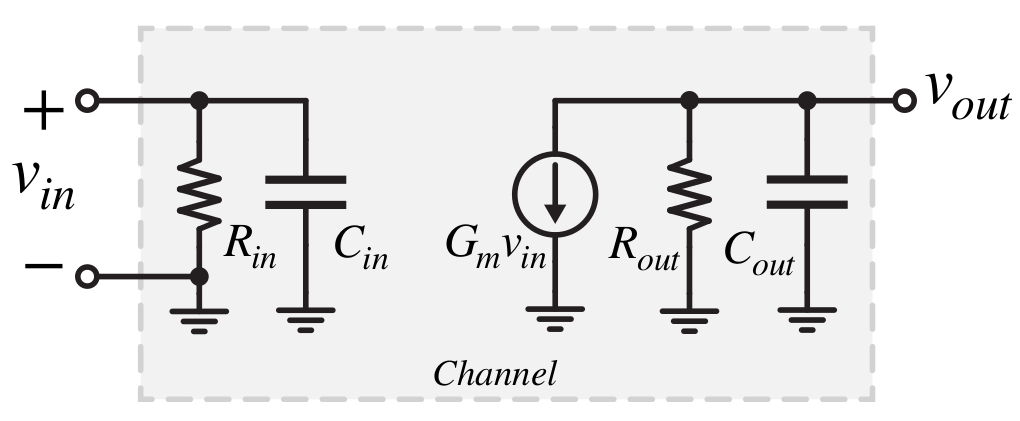
\includegraphics[scale=0.35, center]{p1a1.PNG}\\

The value of the components in the model are listed below.:

    \begin{table}[H]
    \centering
    \setlength{\tabcolsep}{20pt}
    \renewcommand{\arraystretch}{1.5}
        \begin{tabular}{|l|c|}
            \hline
            $R_{in}$ & $1\,M \Omega$\\
            \hline
            $C_{in}$ & $20\,pF$\\
            \hline
            $G_{in}$ & $10\,mS$\\
            \hline
            $R_{out}$ & $10\,k \Omega$\\
            \hline
            $C_{out}$ & $4\,pF$\\
            \hline
        \end{tabular}
    \end{table}

\noindent
\textbf{\emph{Find: }} The following for each circuit:

\begin{enumerate}[label=(\roman*)]
    \item
    {
    Using the model shown in \textit{Fig. 2}, set the value of $R_{probe}$ such that the impedance looking into the probe tip is $10\,M \Omega$ at DC.
    
    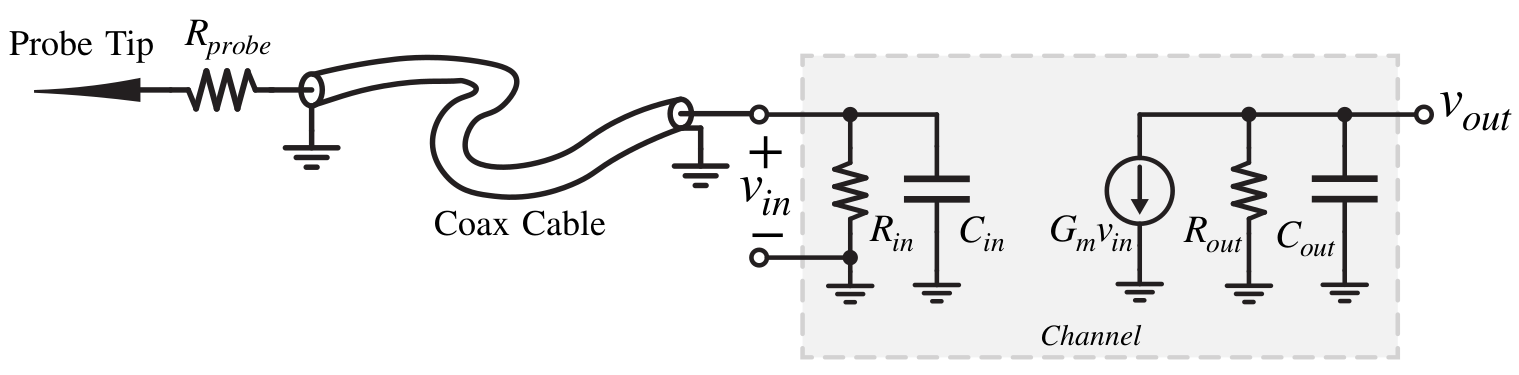
\includegraphics[scale=0.35, center]{p1f1.PNG}\\
    }
    \item
    {
    Find the transfer function for the input voltage of the probe tip to the output of the amplifier.
    \begin{equation*}
        H(s) = \frac{v_{out}(s)}{v_{tip}(s)}
    \end{equation*}
    }
    \item
    {
    What time constant limits the bandwidth of this transfer function?
    }
    \item
    {
    As an update to your design, you decide to add a parallel capacitor ($C_{probe}$) to the $R_{probe}$ as shown in \textit{Fig. 3}. Using the value of $R_{probe}$ from part (\textit{a}), determine the size of $C_{probe}$ such that $\frac{v_{in}(s)}{v_{tip}(s)}$ has an all-pass response.
    
    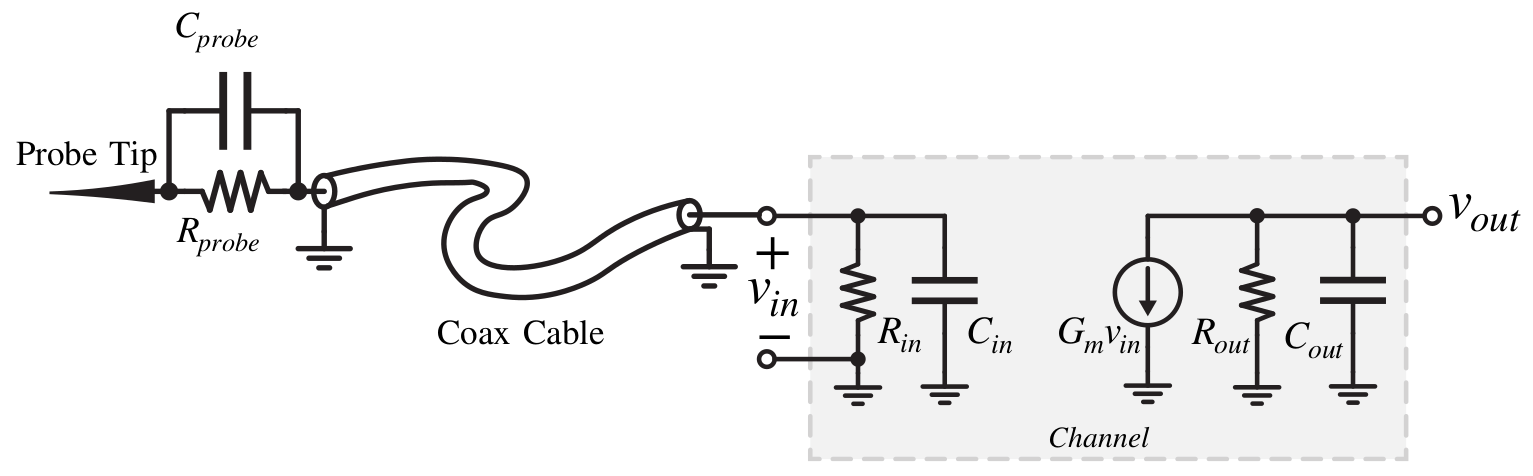
\includegraphics[scale=0.35, center]{p1f2.PNG}\\
    }
    \item
    {
    Now, what is the $-3\,dB$ bandwidth of the new probe/channel combination?
    }
\end{enumerate}

\newpage
\noindent
\textbf{\emph{Solution: }}

\begin{enumerate}[label=(\roman*)]
    %%%%%%%%%%%%%%%%%%
    %%% SOLUTION A %%%
    %%%%%%%%%%%%%%%%%%
    \item
    {
    Below is a schematic of applying a test source at DC to find the input resistance:

    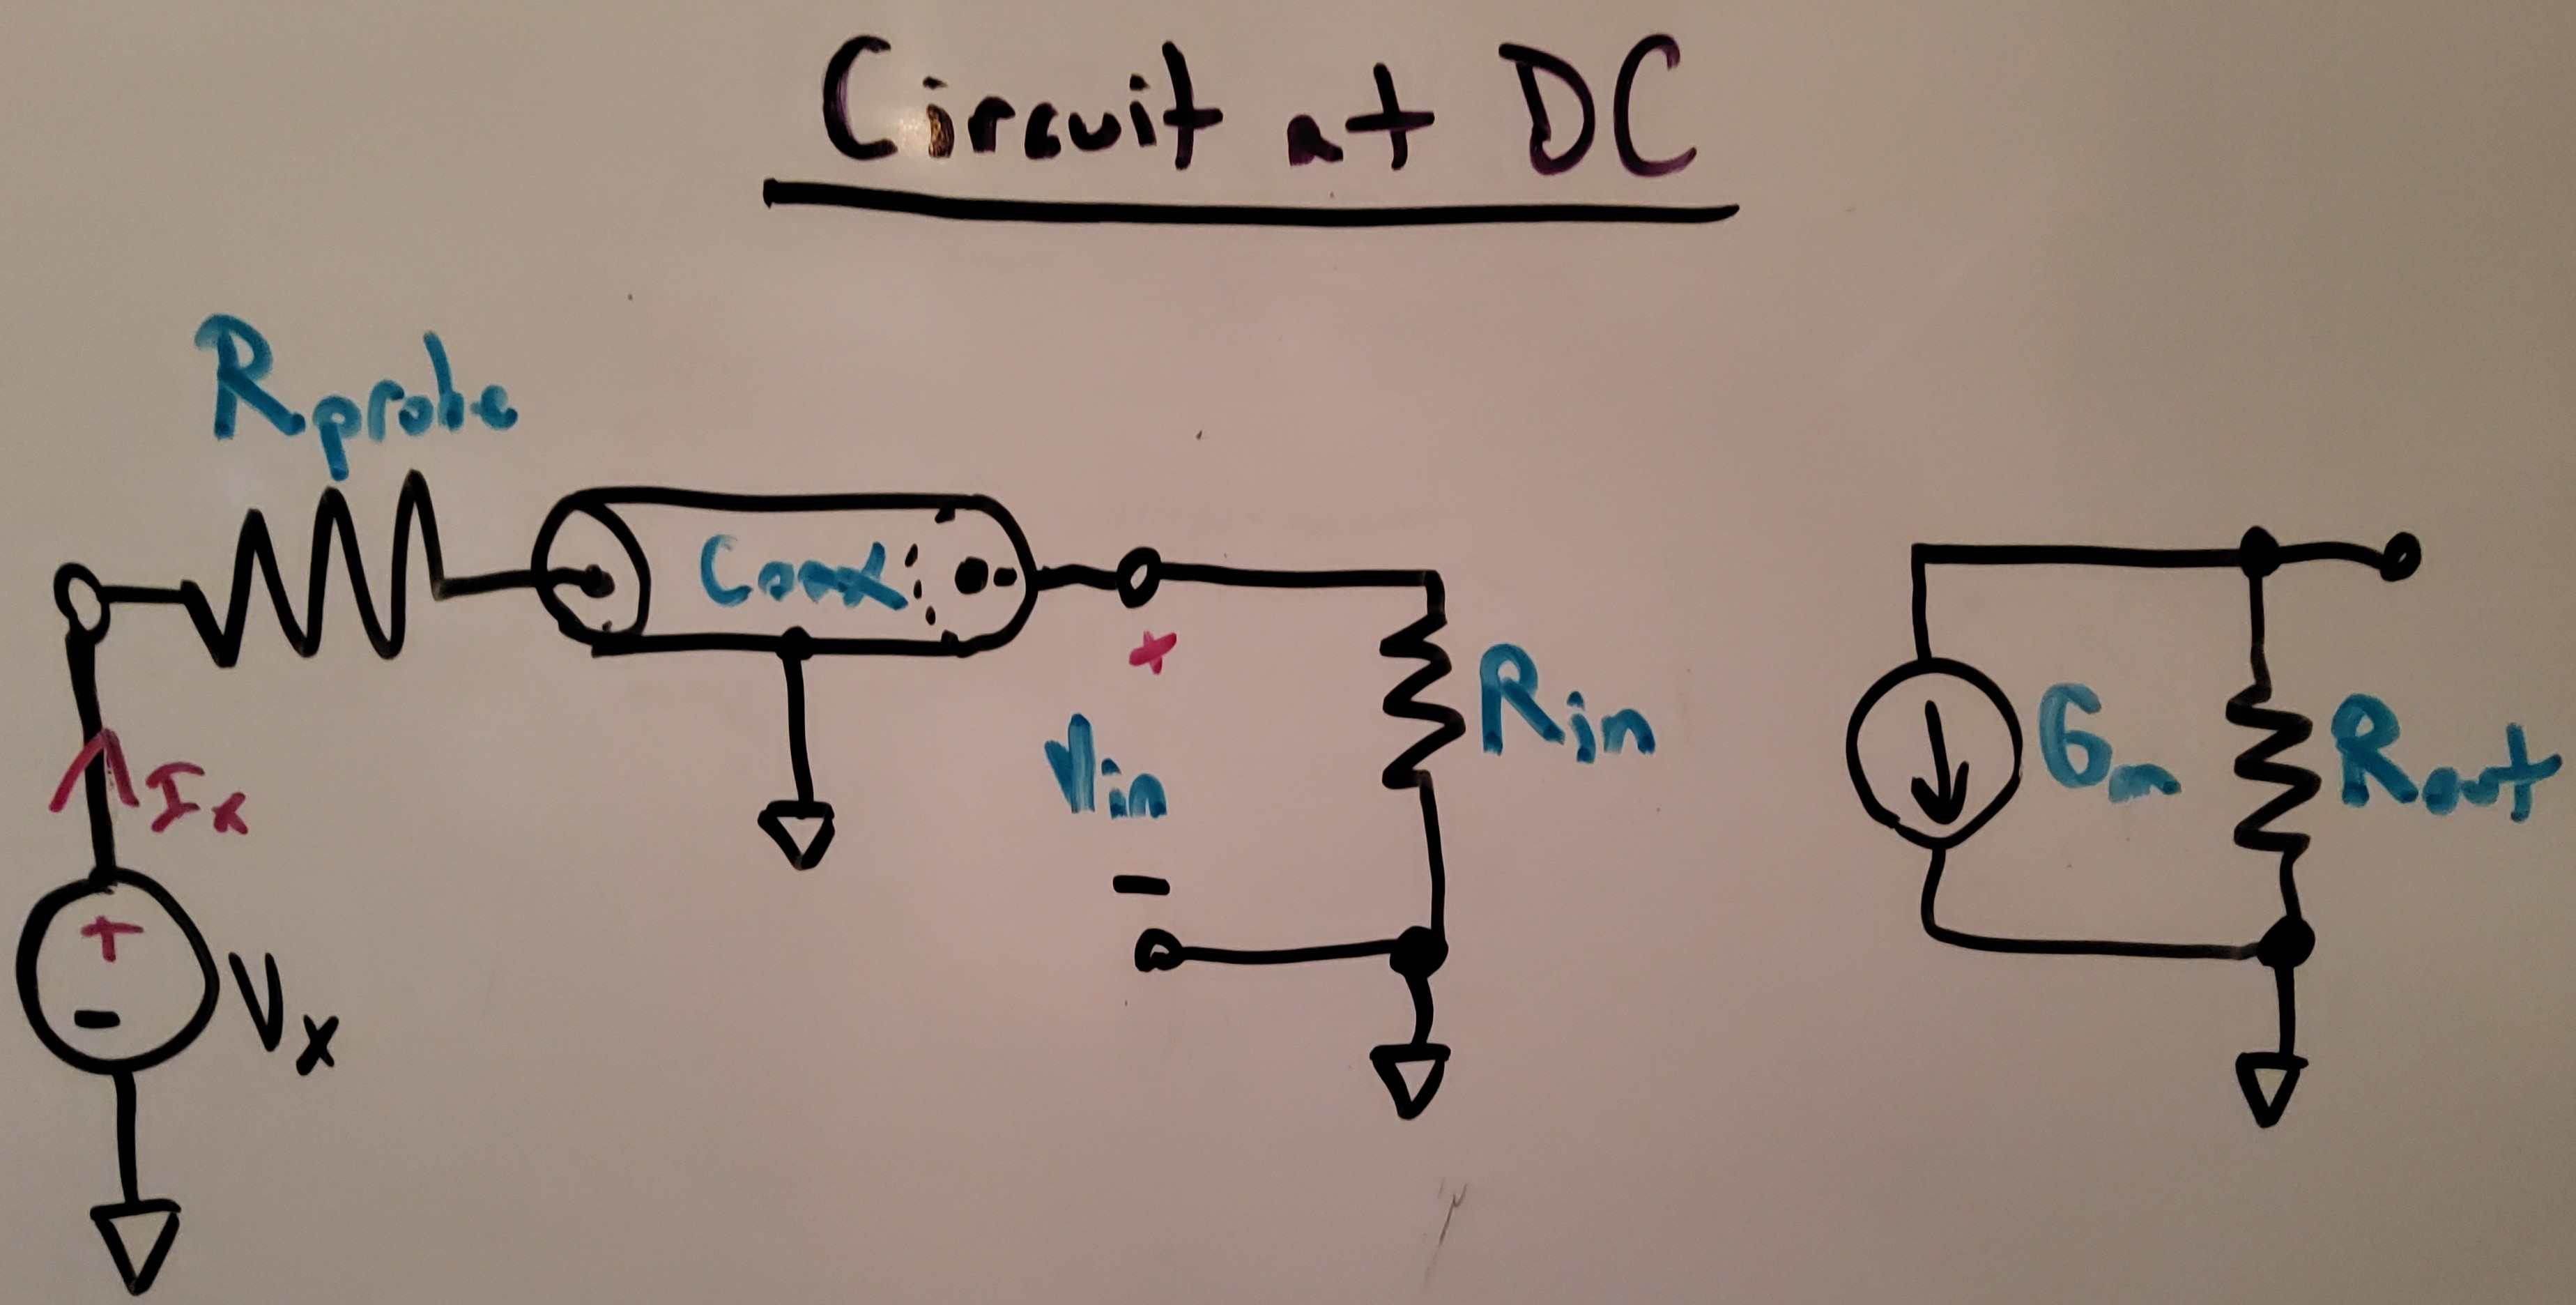
\includegraphics[scale=0.1, center]{p1a1.jpg}\\

    We have that $I_X = V_X/(R_{probe} + R_{in})$, which means that $R_X = R_{probe} + R_{in} = 10\,M\Omega$.  Since we are given that $R_{in} = 1\,M\Omega$, the solution is trivial.\\[0.5cm]    
    $\therefore \quad \boxed{R_{probe} \approx 9\,M\Omega}$
    }
    %%%%%%%%%%%%%%%%%%
    %%% SOLUTION B %%%
    %%%%%%%%%%%%%%%%%%
    \item
    {
    Below is a schematic of the circuit in the frequency domain for analysis of the transfer function:

    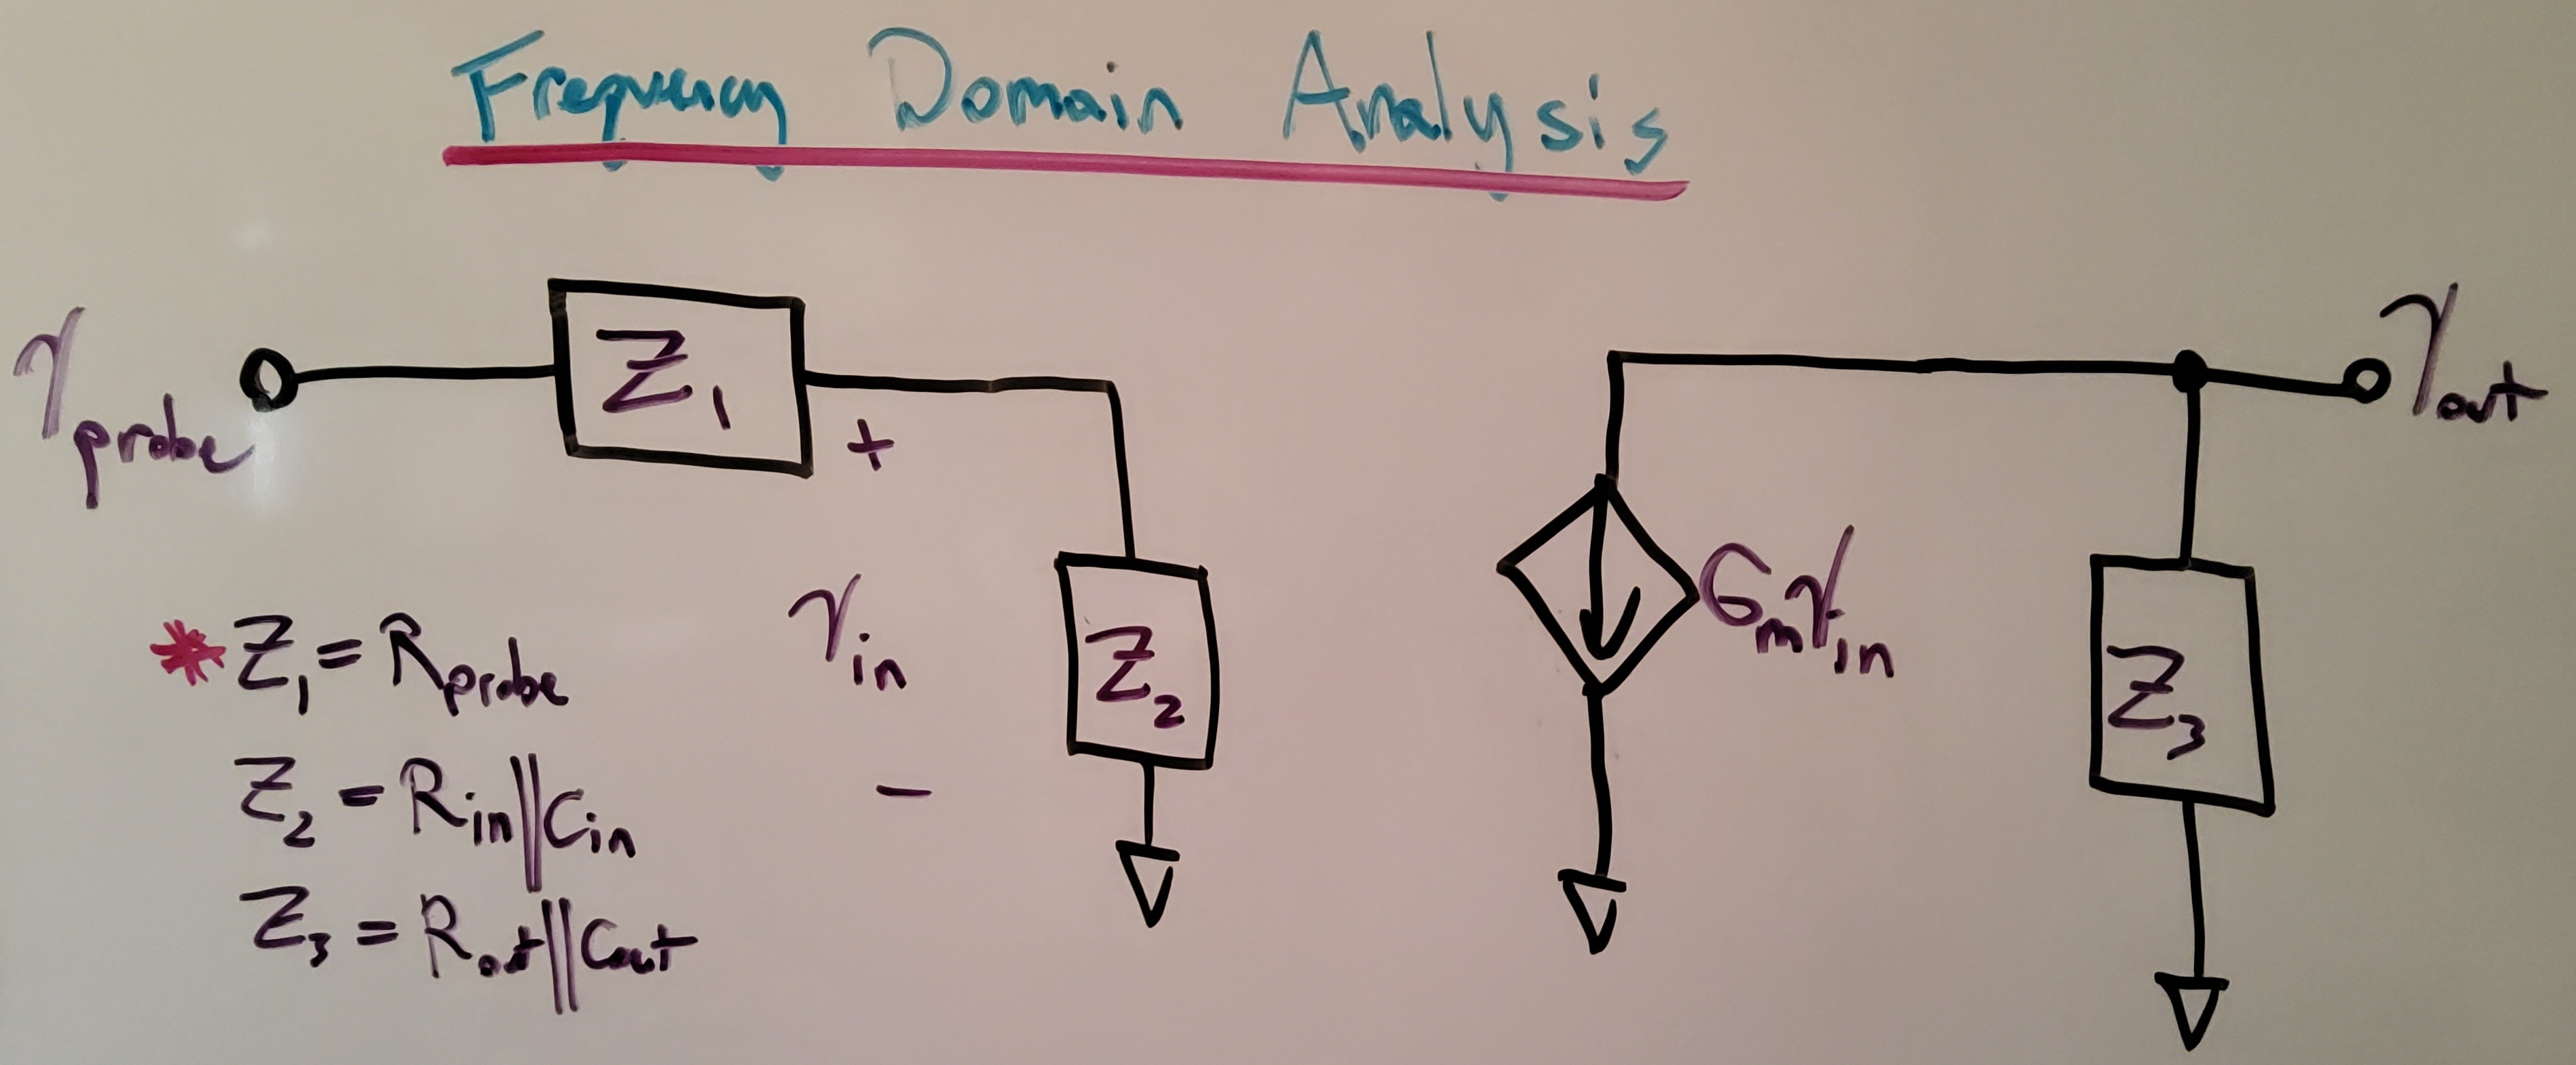
\includegraphics[scale=0.125, center]{p1fd.jpg}\\
    
    To begin, we see that $v_{in}$ forms a voltage divider:
    \begin{align*}
        v_{in} &= v_{tip}\left(\frac{Z_2}{Z_1 + Z_2}\right)
    \end{align*}
    
    Nodal analysis at the output and substitution of $v_{in}$ yields:
    \begin{align*}
        0 &= \frac{v_{out}}{Z_3} + G_m v_{in}\\[0.25cm]
        \implies  v_{out} &= - G_m Z_3 \left[v_{tip}\left(\frac{Z_2}{Z_1 + Z_2}\right)\right]\\[0.25cm]
        \implies  \frac{v_{out}}{v_{tip}} &= - G_m\left(\frac{Z_2 Z_3}{Z_1 + Z_2}\right)\\[0.25cm]
        &= - G_m\left(\frac{R_{in} \parallel C_{in} \cdot R_{out} \parallel C_{out}}{R_{probe} + R_{in} \parallel C_{in}}\right)\\[0.25cm]
        &= - G_m\left[\frac{\left(\frac{R_{in}}{1 + s R_{in} C_{in}}\right) \cdot \left(\frac{R_{out}}{1 + s R_{out} C_{out}}\right)}
                {R_{probe} + \left(\frac{R_{in}}{1 + s R_{in} C_{in}}\right)}\right]\\[0.25cm]
        &= - G_m\left[\left(\frac{R_{in} \cdot R_{out}}{\cancel{(1 + s R_{in} C_{in})}(1 + s R_{out} C_{out})}\right)
                    \cdot \left(\frac{\cancel{(1 + s R_{in} C_{in})}}{R_{in} + R_{probe}(1 + s R_{in} C_{in})}\right)\right]\\[0.25cm]
        &= -\left[\frac{G_m R_{in} R_{out}}{(1 + s R_{out} C_{out})(R_{in} + R_{probe} + s R_{in} R_{probe} C_{in})}\right]
    \end{align*}

    Thus, our final simplified expression for the transfer function:
    \begin{equation}
        \boxed{\frac{v_{out}(s)}{v_{tip}(s)} = -\left(\frac{G_m R_{in} R_{out}}{R_{in} + R_{probe}}\right)\left[\frac{1}{(1 + s R_{in} \parallel R_{probe} C_{in})(1 + s R_{out} C_{out})}\right]}
    \end{equation}
    }
    %%%%%%%%%%%%%%%%%%
    %%% SOLUTION C %%%
    %%%%%%%%%%%%%%%%%%
    \item
    {
    We have two poles that determine the bandwidth in our circuit:
    \begin{align}
        f_{P_1} &= \frac{1}{2\pi R_{in} \parallel R_{probe} C_{in}}\\[0.25cm]
        f_{P_2} &= \frac{1}{2\pi R_{out} C_{out}}
    \end{align}
    
    Plugging in the given numerical values yields:
    \begin{align}
        f_{P_1} &\approx 8750\,Hz\\[0.25cm]
        f_{P_2} &\approx 4\,MHz
    \end{align}
    
    The first pole at the lower frequency limits the bandwidth of this filter.
    }
    \newpage
    %%%%%%%%%%%%%%%%%%
    %%% SOLUTION D %%%
    %%%%%%%%%%%%%%%%%%
    \item
    {
    Now the only change from our previous transfer function is that $Z_1 = R_{probe} \parallel C_{probe}$.  First let's substitute for $v_{out}$ of the transfer function we found earlier:
    
    \begin{align*}
        \frac{v_{out}}{v_{tip}} &= \cancel{-G_m}\left(\frac{Z_2 \cancel{Z_3}}{Z_1 + Z_2}\right) = \frac{\cancel{-G_m Z_3} v_{in}}{v_{tip}}\\[0.25cm]
        \implies \frac{v_{in}}{v_{tip}} &= \frac{Z_2}{Z_1 + Z_2}\\[0.25cm]
        &= \frac{\frac{R_{in}}{1 + s R_{in} C_{in}}}{\frac{R_{probe}}{1 + s R_{probe} C_{probe}} + \frac{R_{in}}{1 + s R_{in} C_{in}}}\\[0.25cm]
        &= \frac{R_{in}}{\cancel{1 + s R_{in} C_{in}}}\left[\frac{(1 + s R_{probe} C_{probe})\cancel{(1 + s R_{in} C_{in})}}{R_{probe}(1 + s R_{in} C_{in}) + R_{in}(1 + s R_{probe} C_{probe})}\right]\\[0.25cm]
        &= \frac{R_{in}(1 + s R_{probe} C_{probe})}{R_{probe}(1 + s R_{in} C_{in}) + R_{in}(1 + s R_{probe} C_{probe})}\\[0.25cm]
    \end{align*}
    
    The only possible value of $C_{probe}$ that will allow an all-pass filter is one large enough to dominate the other pole.  Let's take a limit to show this will work:
    \begin{align*}
        \lim_{C_{probe}\to\infty} &\; \frac{R_{in}(1 + s R_{probe} C_{probe})}{R_{probe}(1 + s R_{in} C_{in}) + R_{in}(1 + s R_{probe} C_{probe})}\\[0.25cm]
        &= \frac{R_{in}(1 + s R_{probe} \infty)}{R_{probe}(1 + s R_{in} C_{in}) + R_{in}(1 + s R_{probe} \infty)}\\[0.25cm]
        &= \cancelto{1}{\frac{R_{in}(\infty)}{R_{in}(\infty)}}
    \end{align*}
    
    $\therefore \quad \boxed{C_{probe} \gg C_{in} \approx \infty}$
    }
    \vspace{1cm}
    %%%%%%%%%%%%%%%%%%
    %%% SOLUTION E %%%
    %%%%%%%%%%%%%%%%%%
    \item
    {
    Since this is an all-pass filter, it has an infinite bandwidth, meaning that it provides a gain of 1 for all frequencies.
    }
\end{enumerate}
%%%%%%%%%%%%%%%%%%%%%%%%%%%%%%%%%%%%%%%%%%%%%%%%%%%%%%%%%%%%%%%%%%%%%%%%%%%%%%%%%%%%%%%%%%%%%%%%%%%%%%%%%%%
%                                           QUESTION 2                                                    %
%%%%%%%%%%%%%%%%%%%%%%%%%%%%%%%%%%%%%%%%%%%%%%%%%%%%%%%%%%%%%%%%%%%%%%%%%%%%%%%%%%%%%%%%%%%%%%%%%%%%%%%%%%%
\newpage
\section{Continuous Time Linear Equalizer}
\textbf{\emph{Given: }} Shown in \textit{Fig. 4} is a circuit that is commonly used in high-speed serial link applications to enhance the gain at higher frequencies. Assume $\lambda = 0$, $\gamma = 0$.

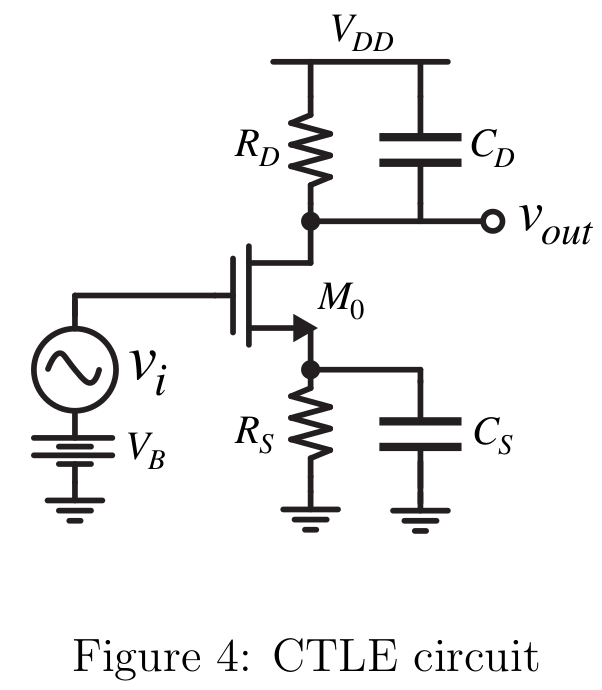
\includegraphics[scale=0.25, center]{p2f4.PNG}\\
\textbf{\emph{Find: }} The following:

\begin{enumerate}[label=(\alph*)]
    \item
    {
    Draw the small signal model of the circuit. Neglect all capacitances except explicitly shown in the diagram.
    }
    \item
    {
    The bode plot below represents the transfer function of the above circuit. Determine the pole/zero locations based on the bode plot and find the transfer function of the circuit. Assume all zeros are in the left half-plane (LHP).
    }
    \item
    {
    Find the values, labeled as $X$ (in $dB$) and $Y$ (in $Hz$) from the bode plot in \textit{Fig. 5}
    
    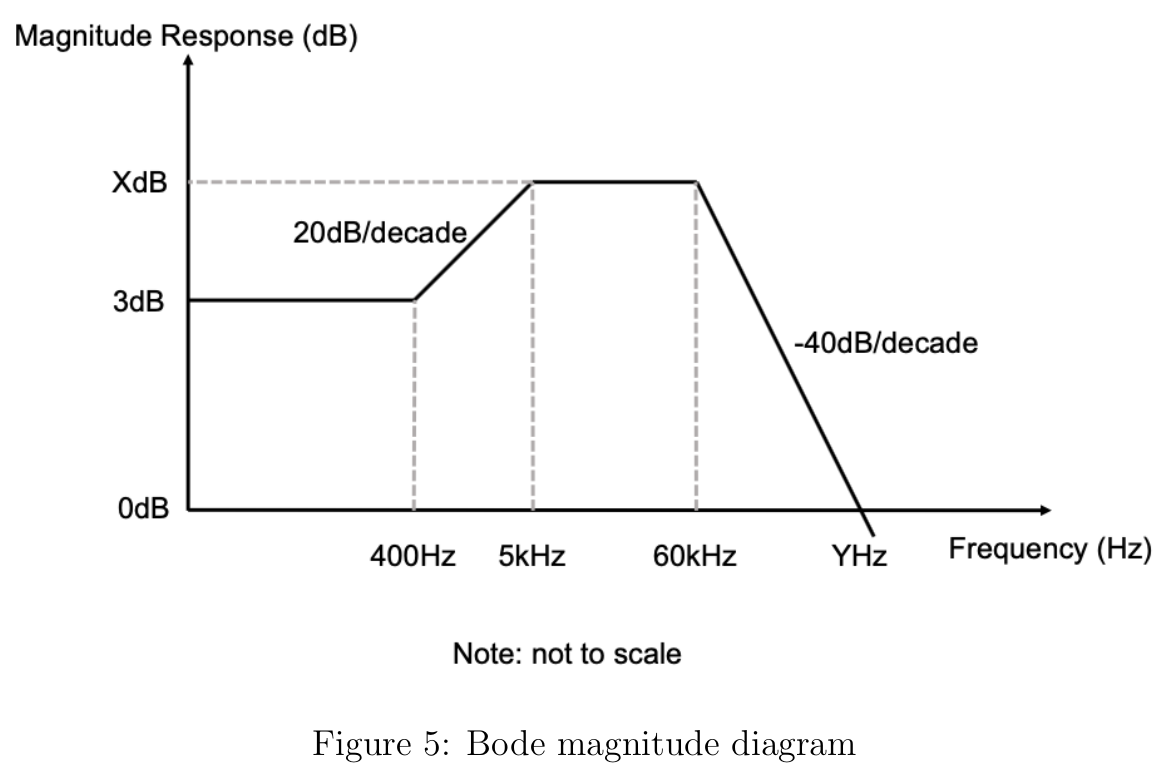
\includegraphics[scale=0.3, center]{p2f5.PNG}\\
    }
    \item
    {
    Which capacitor shown in the circuit causes the zero to appear in the frequency response? Why? Please explain your answers qualitatively.
    }
\end{enumerate}
\newpage
\noindent
\textbf{\emph{Solution: }}

\begin{enumerate}[label=(\alph*)]
    %%%%%%%%%%%%%%%%%%
    %%% SOLUTION A %%%
    %%%%%%%%%%%%%%%%%%
    \item
    {
    Below is a schematic of the small-signal model:

    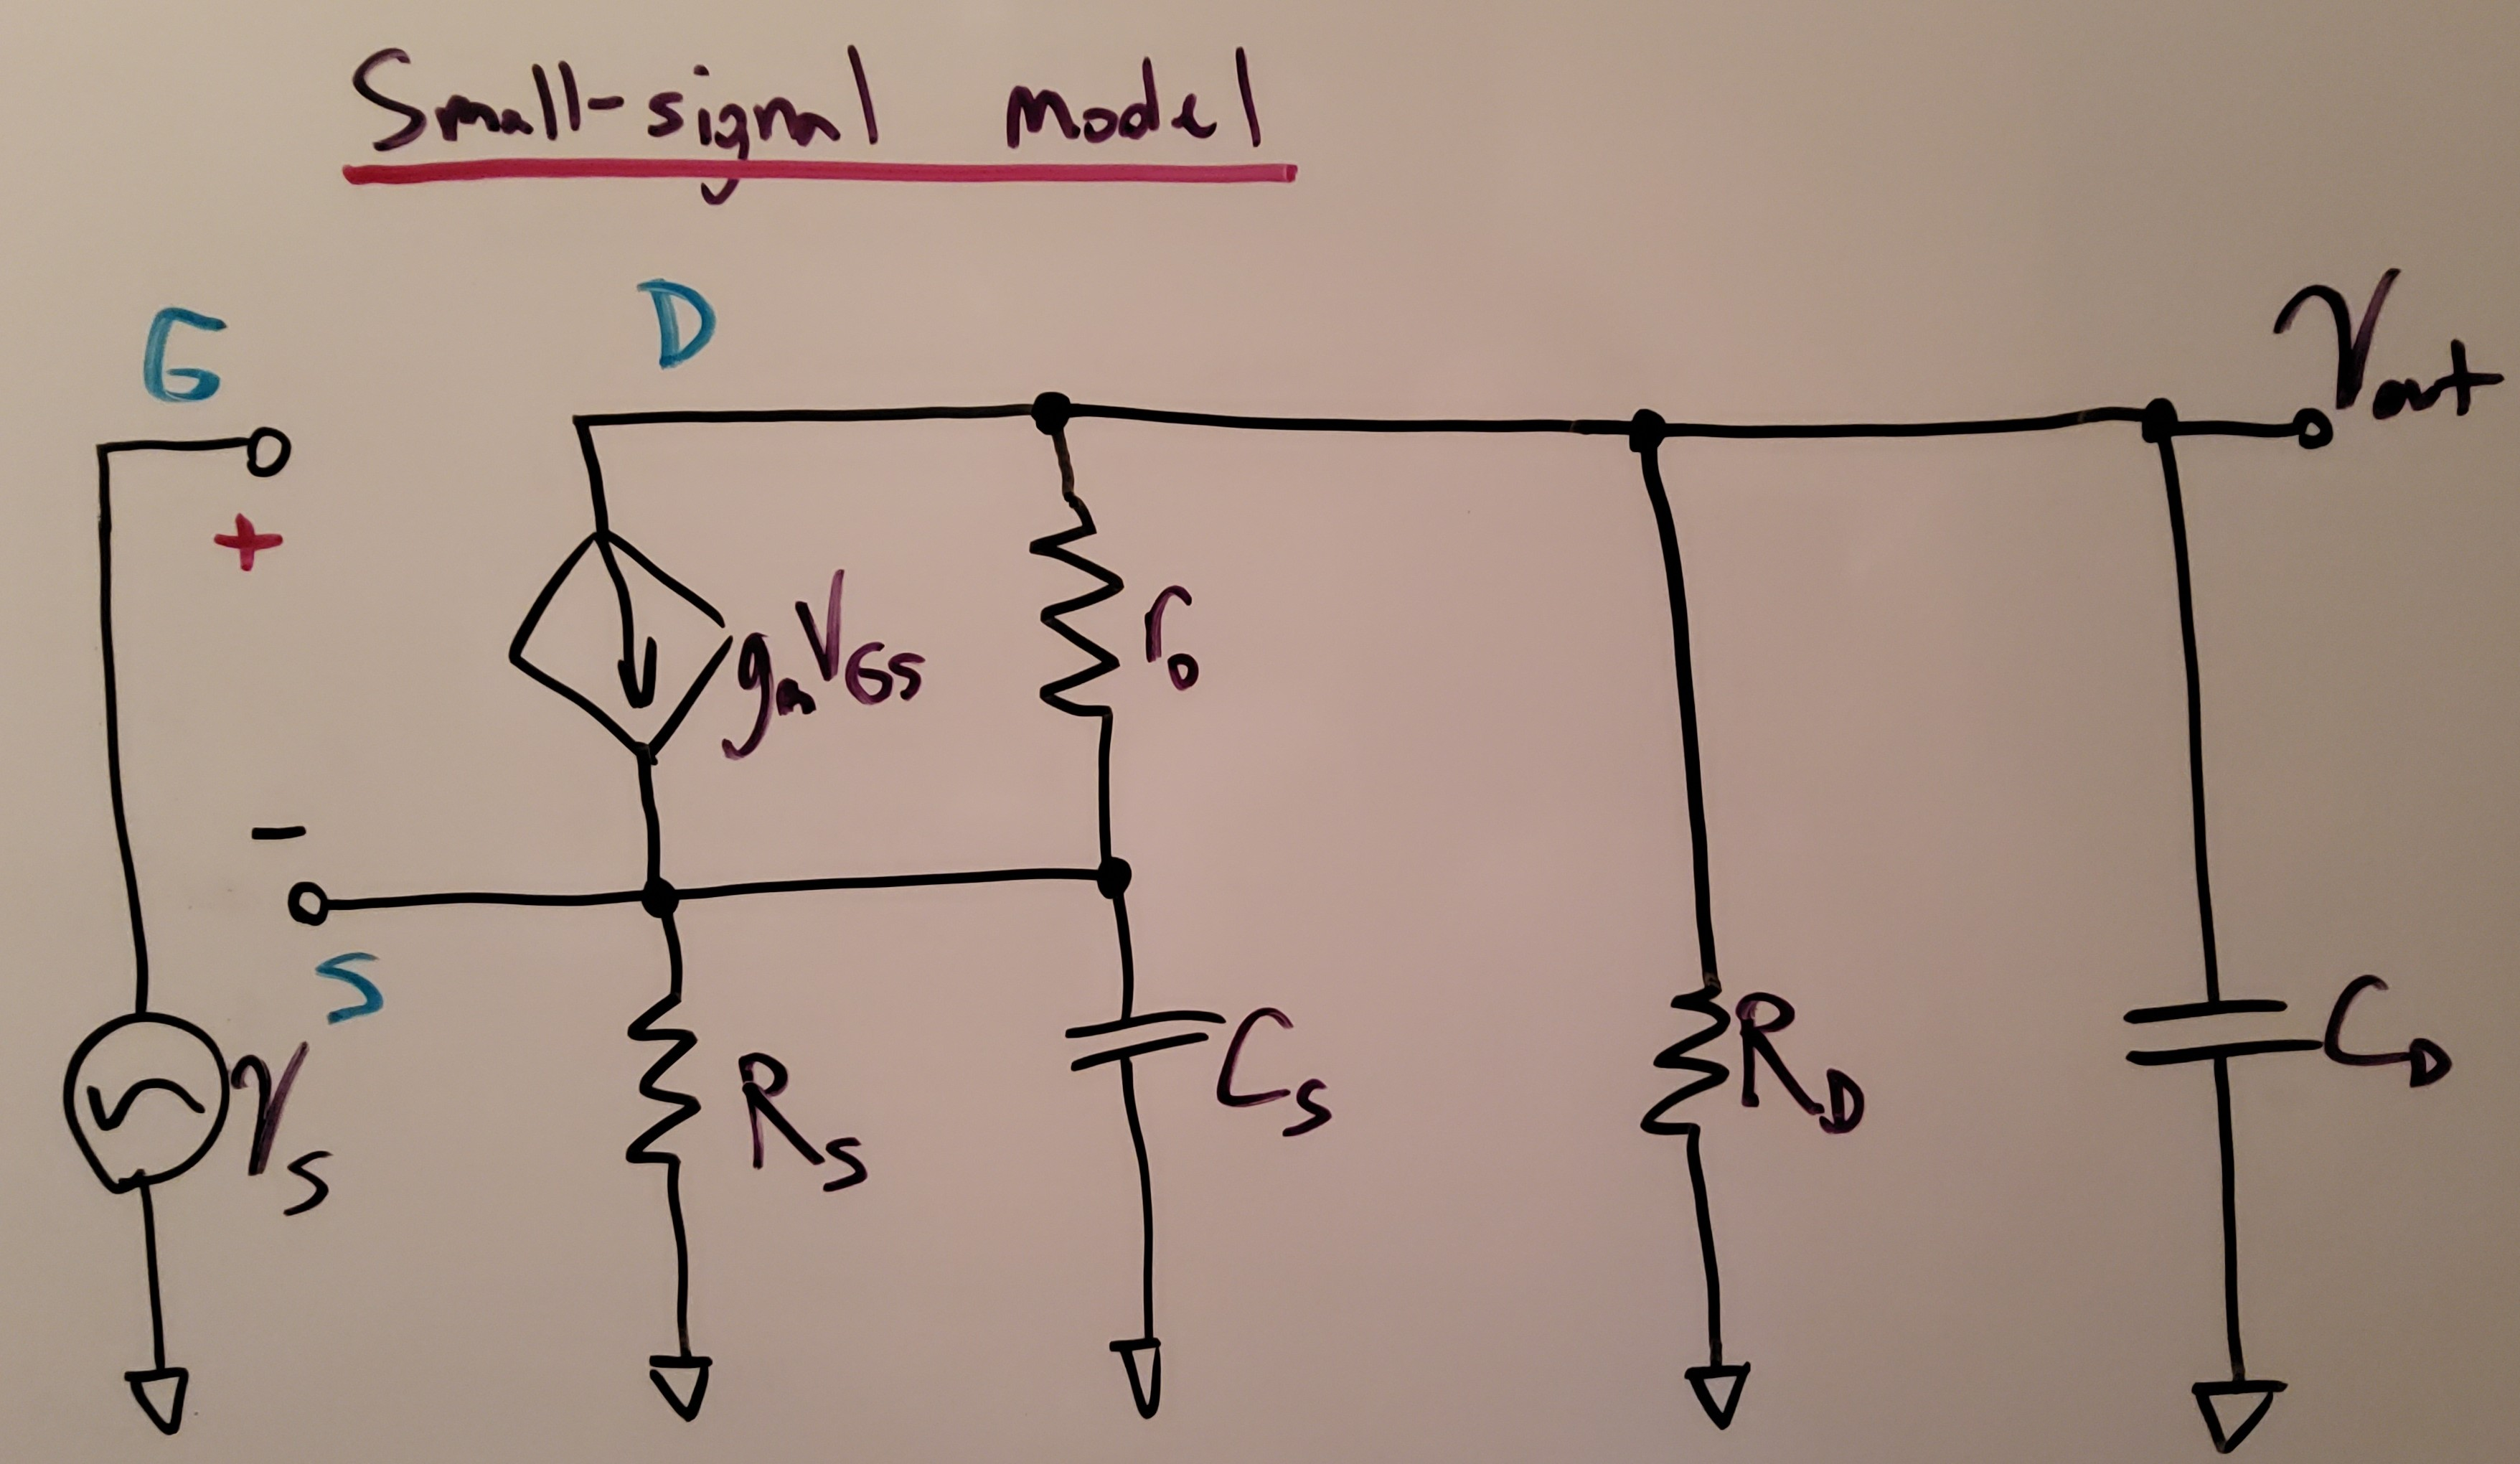
\includegraphics[scale=0.08, center]{p2ss.jpg}\\
    }
    %%%%%%%%%%%%%%%%%%
    %%% SOLUTION B %%%
    %%%%%%%%%%%%%%%%%%
    \item
    {
    There is a zero at $400\,Hz$, the first pole at $5\,kHz$, and a pole with a multiplicity of two at $60\,kHz$.\\[0.5cm]
    
    The DC gain is $3\,dB$, then we have $20\,\log(A_0) = 3$.  Rearranging:
    \begin{equation}
        A_0 = 10^{\frac{3}{20}} = \sqrt{2}
    \end{equation}
    
    By inspection, the transfer function is:
    \begin{equation}
        \boxed{H(s) = \mathlarger{\mathlarger{\sqrt{2} \left[\frac{(1 + \frac{s}{2\pi \cdot 400\,Hz})}{(1 + \frac{s}{2\pi \cdot 5\,kHz}){(1 + \frac{s}{2\pi \cdot 60\,kHz})}^2}\right]}}}
    \end{equation}
    }
    %%%%%%%%%%%%%%%%%%
    %%% SOLUTION C %%%
    %%%%%%%%%%%%%%%%%%
    \item
    {
    For $X$, we find the amount of decade increase using the law of logs:
    
    \begin{align*}
        X &= 3\,dB + 20\,dB(\log_{10}(5000) - \log_{10}(400)) = 3\,dB + 20\,dB(1.0969)\\[0.25cm]
        \implies \Aboxed{X &= 24.94\,dB}
    \end{align*}
    
    For $Y$, we use the equation of a slope and have:
    
    \begin{equation}
        X_f - X_0 = m(Y_f - Y_0) \implies -24.94\,dB = -40\,dB/dec(\log_{10}(Y) - \log_{10}(60k))
    \end{equation}
    
    Rearranging, we have:
    
    \begin{align*}
        1 &= -15.06\,\log(Y) + 64.94\,\log(60\,k)\\[0.25cm]
        \implies &\, 15.06\,\log(Y) = 64.94\,\log(60\,k) - 1\\[0.25cm]
        \implies &\, 15.06\,Y = 64.94\,(60\,k) - 10\\[0.25cm]
        \implies \Aboxed{Y &\approx 258725\,Hz}
    \end{align*}
    }
    %%%%%%%%%%%%%%%%%%
    %%% SOLUTION D %%%
    %%%%%%%%%%%%%%%%%%
    \item
    {
    $C_S$ causes the zero to appear, and $C_D$ causes the pole to appear.  A zero creates an increase in the slope of the gain, so $C_S$ acting as a wire at lower frequencies in AC conditions allows a larger voltage to appear at the output.  Because $C_D$ acts as a higher frequency pole, when it becomes a wire at its break frequency it allows the amplified current a path to ground and decreases the gain.
    }
\end{enumerate}
%%%%%%%%%%%%%%%%%%%%%%%%%%%%%%%%%%%%%%%%%%%%%%%%%%%%%%%%%%%%%%%%%%%%%%%%%%%%%%%%%%%%%%%%%%%%%%%%%%%%%%%%%%%
%                                           QUESTION 3                                                    %
%%%%%%%%%%%%%%%%%%%%%%%%%%%%%%%%%%%%%%%%%%%%%%%%%%%%%%%%%%%%%%%%%%%%%%%%%%%%%%%%%%%%%%%%%%%%%%%%%%%%%%%%%%%
\newpage
\section{Transimpedance Amplifier}
\textbf{\emph{Given: }} Consider the amplifier shown in \textit{Fig. 6}.  Assume $R_G = 0$.

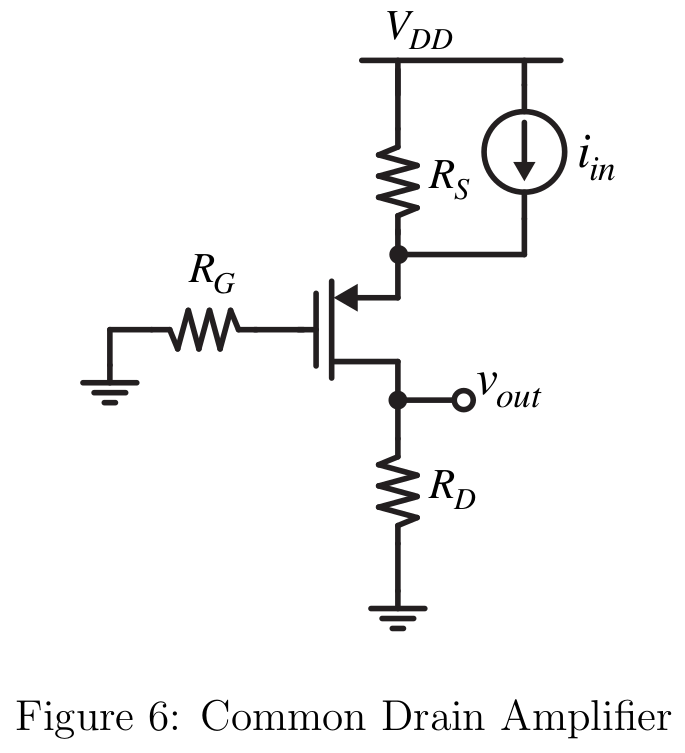
\includegraphics[scale=0.35, center]{p2f6.PNG}\\

\vspace{0.5cm}
\noindent
\textbf{\emph{Find: }} The following:

\begin{enumerate}[label=(\alph*)]
    \item
    {
    Draw the small signal model of the circuit considering both $C_{GS}$ and $C_{GD}$ of the device.
    }
    \item
    {
    Determine the $-3\,dB$ bandwidth of the input-output transfer function using OCTC. Your answer should be symbolic, in terms of the small signal parameters of the device as well as the resistances shown.
    }
    \item
    {
    As the designer, how would you go about setting the value of $R_S$? Try to come up with a constraint on $R_S$ to maximize the gain of the circuit.
    }
    \item
    {
    Qualitatively explain the impact of a non-zero $R_G$ in the $-3\,dB$ bandwidth of the circuit? What value of $R_G$ should maximize this bandwidth?
    }
\end{enumerate}
\newpage
\noindent
\textbf{\emph{Solution: }}

\begin{enumerate}[label=(\alph*)]
    %%%%%%%%%%%%%%%%%%
    %%% SOLUTION A %%%
    %%%%%%%%%%%%%%%%%%
    \item
    {
    Below is a schematic of the small-signal model.  The input current source was transformed to its Thevenin equivalent circuit.  The body transconductance is included, but will be ignored for the subsequent parts:

    \vspace{1cm}
    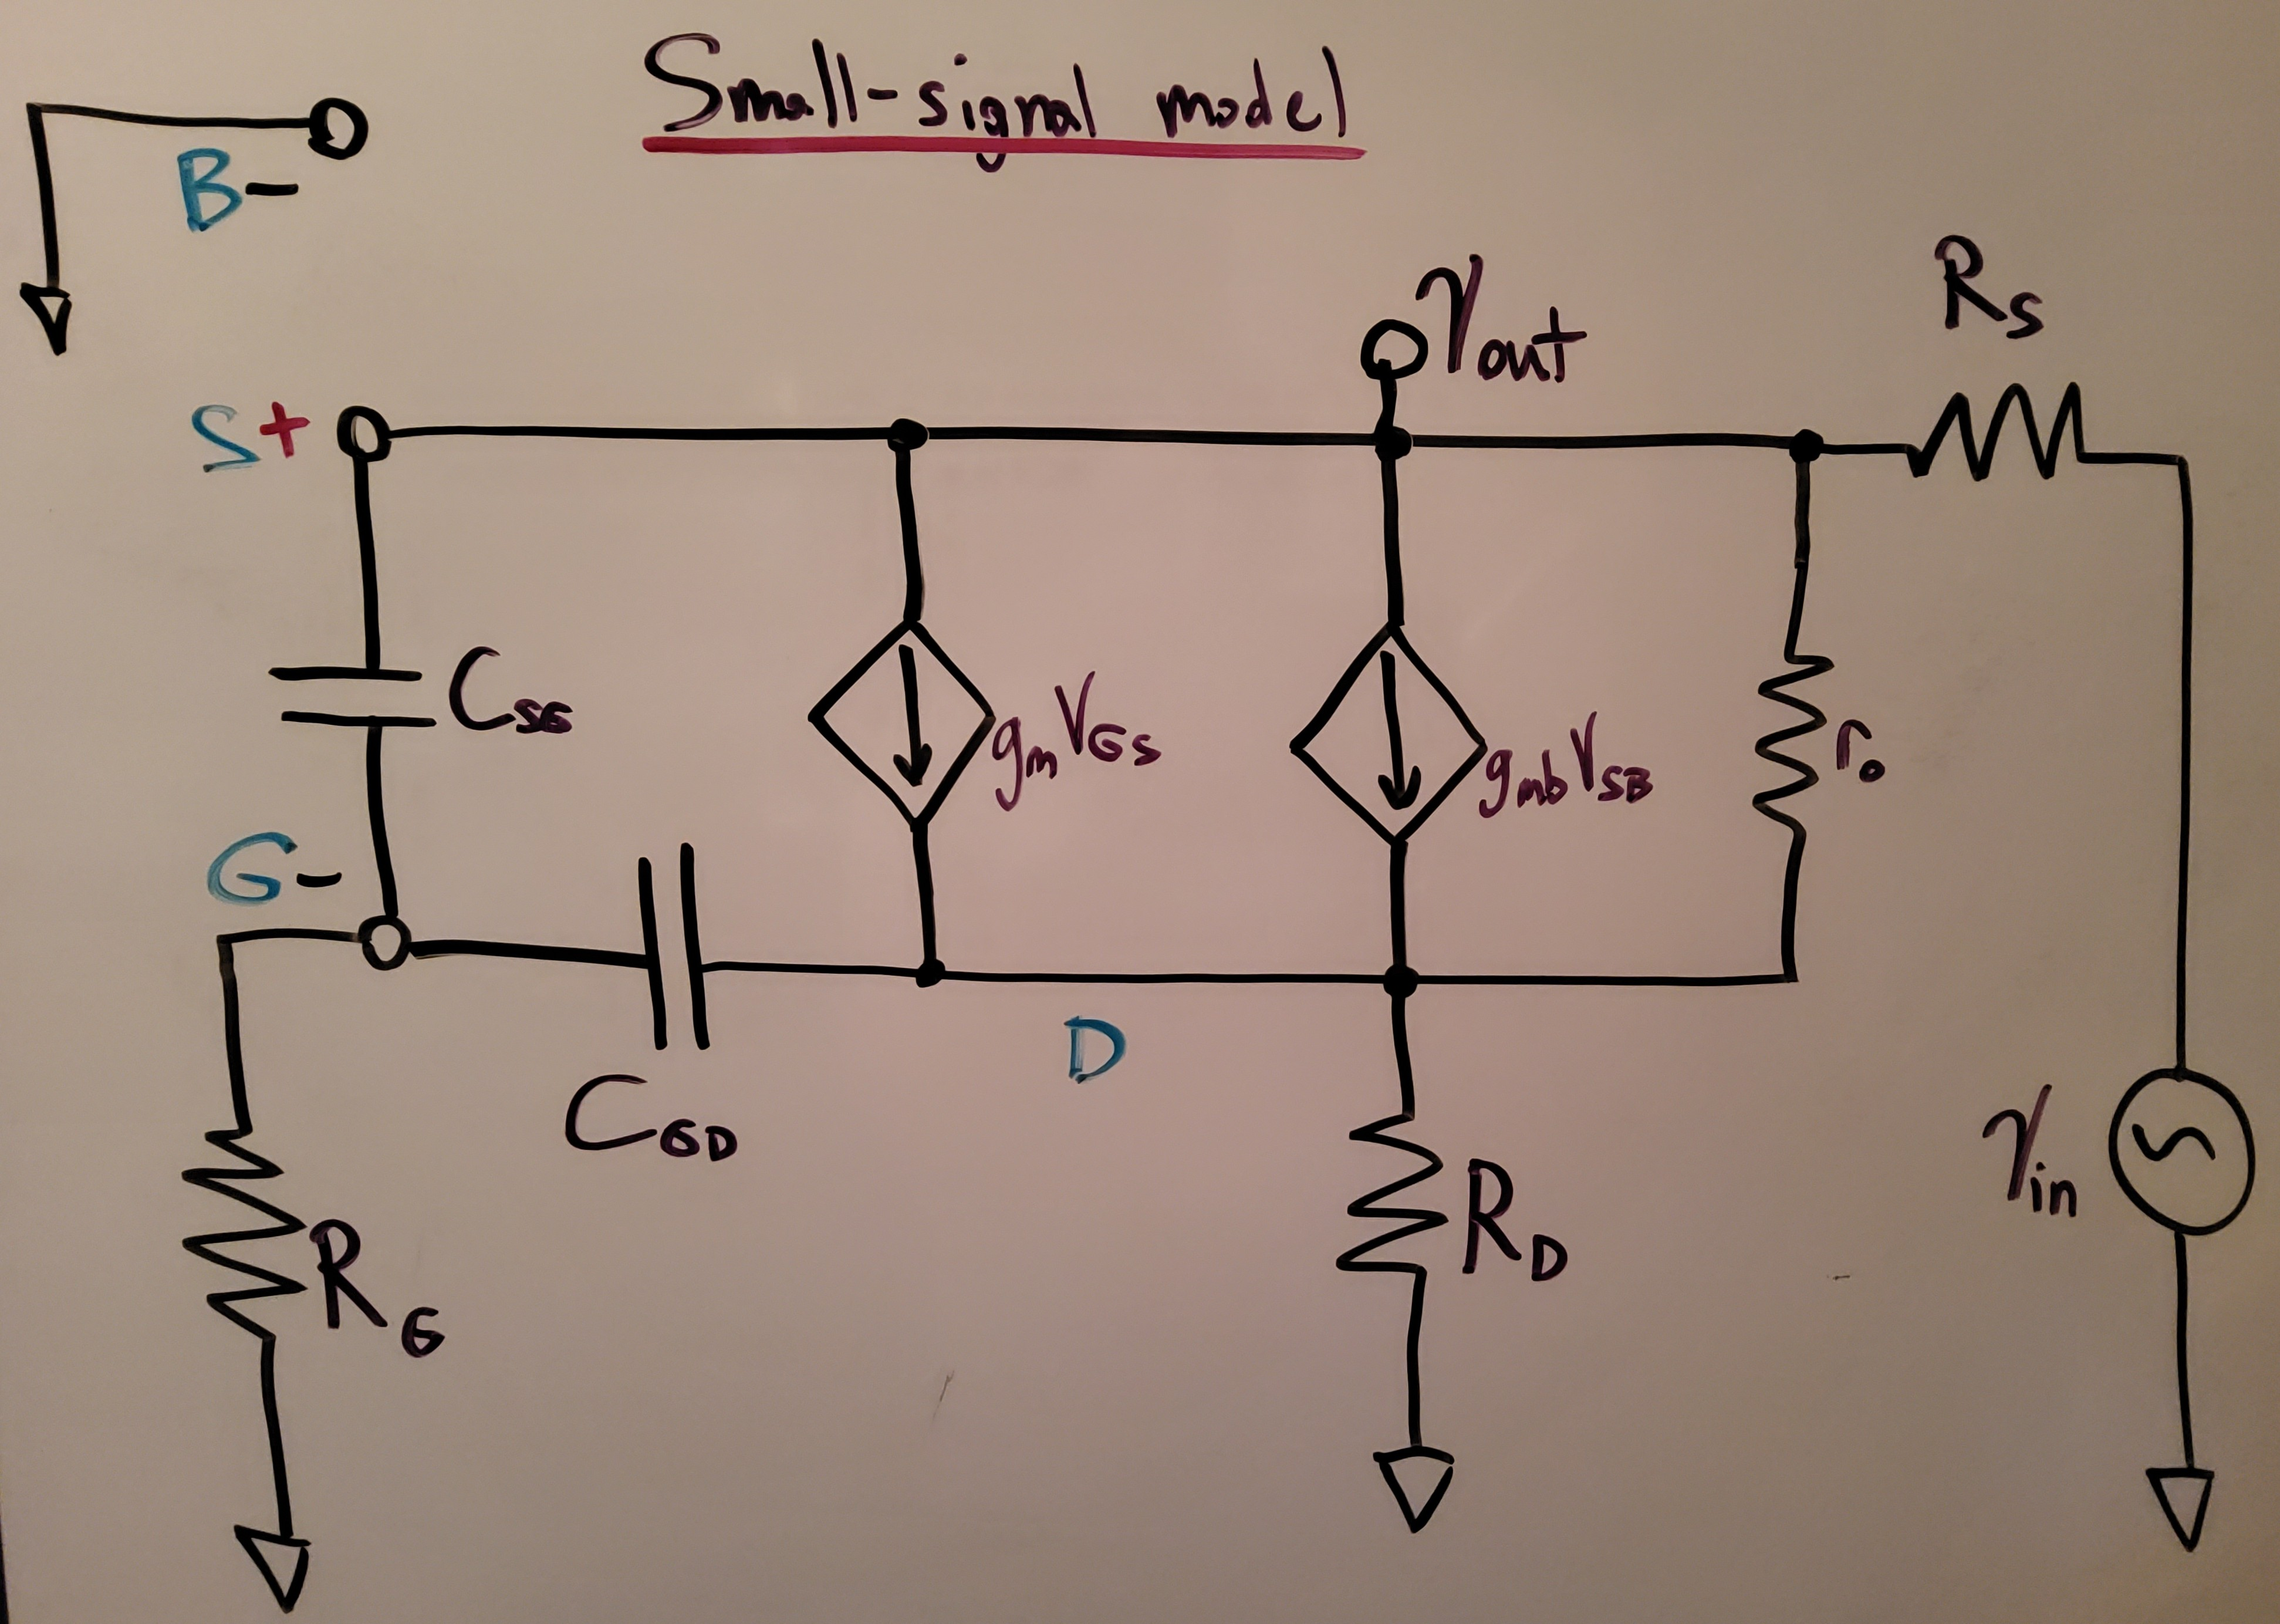
\includegraphics[scale=0.125, center]{p3ss.jpg}\\
    }
    \newpage
    %%%%%%%%%%%%%%%%%%
    %%% SOLUTION B %%%
    %%%%%%%%%%%%%%%%%%
    \item
    {
    \underline{\textbf{OCTC: $C_{SG}$}}\\[0.1cm]
    Below is a schematic of the small-signal model, with all caps opened, and a test source applied in place of $C_{SG}$:

    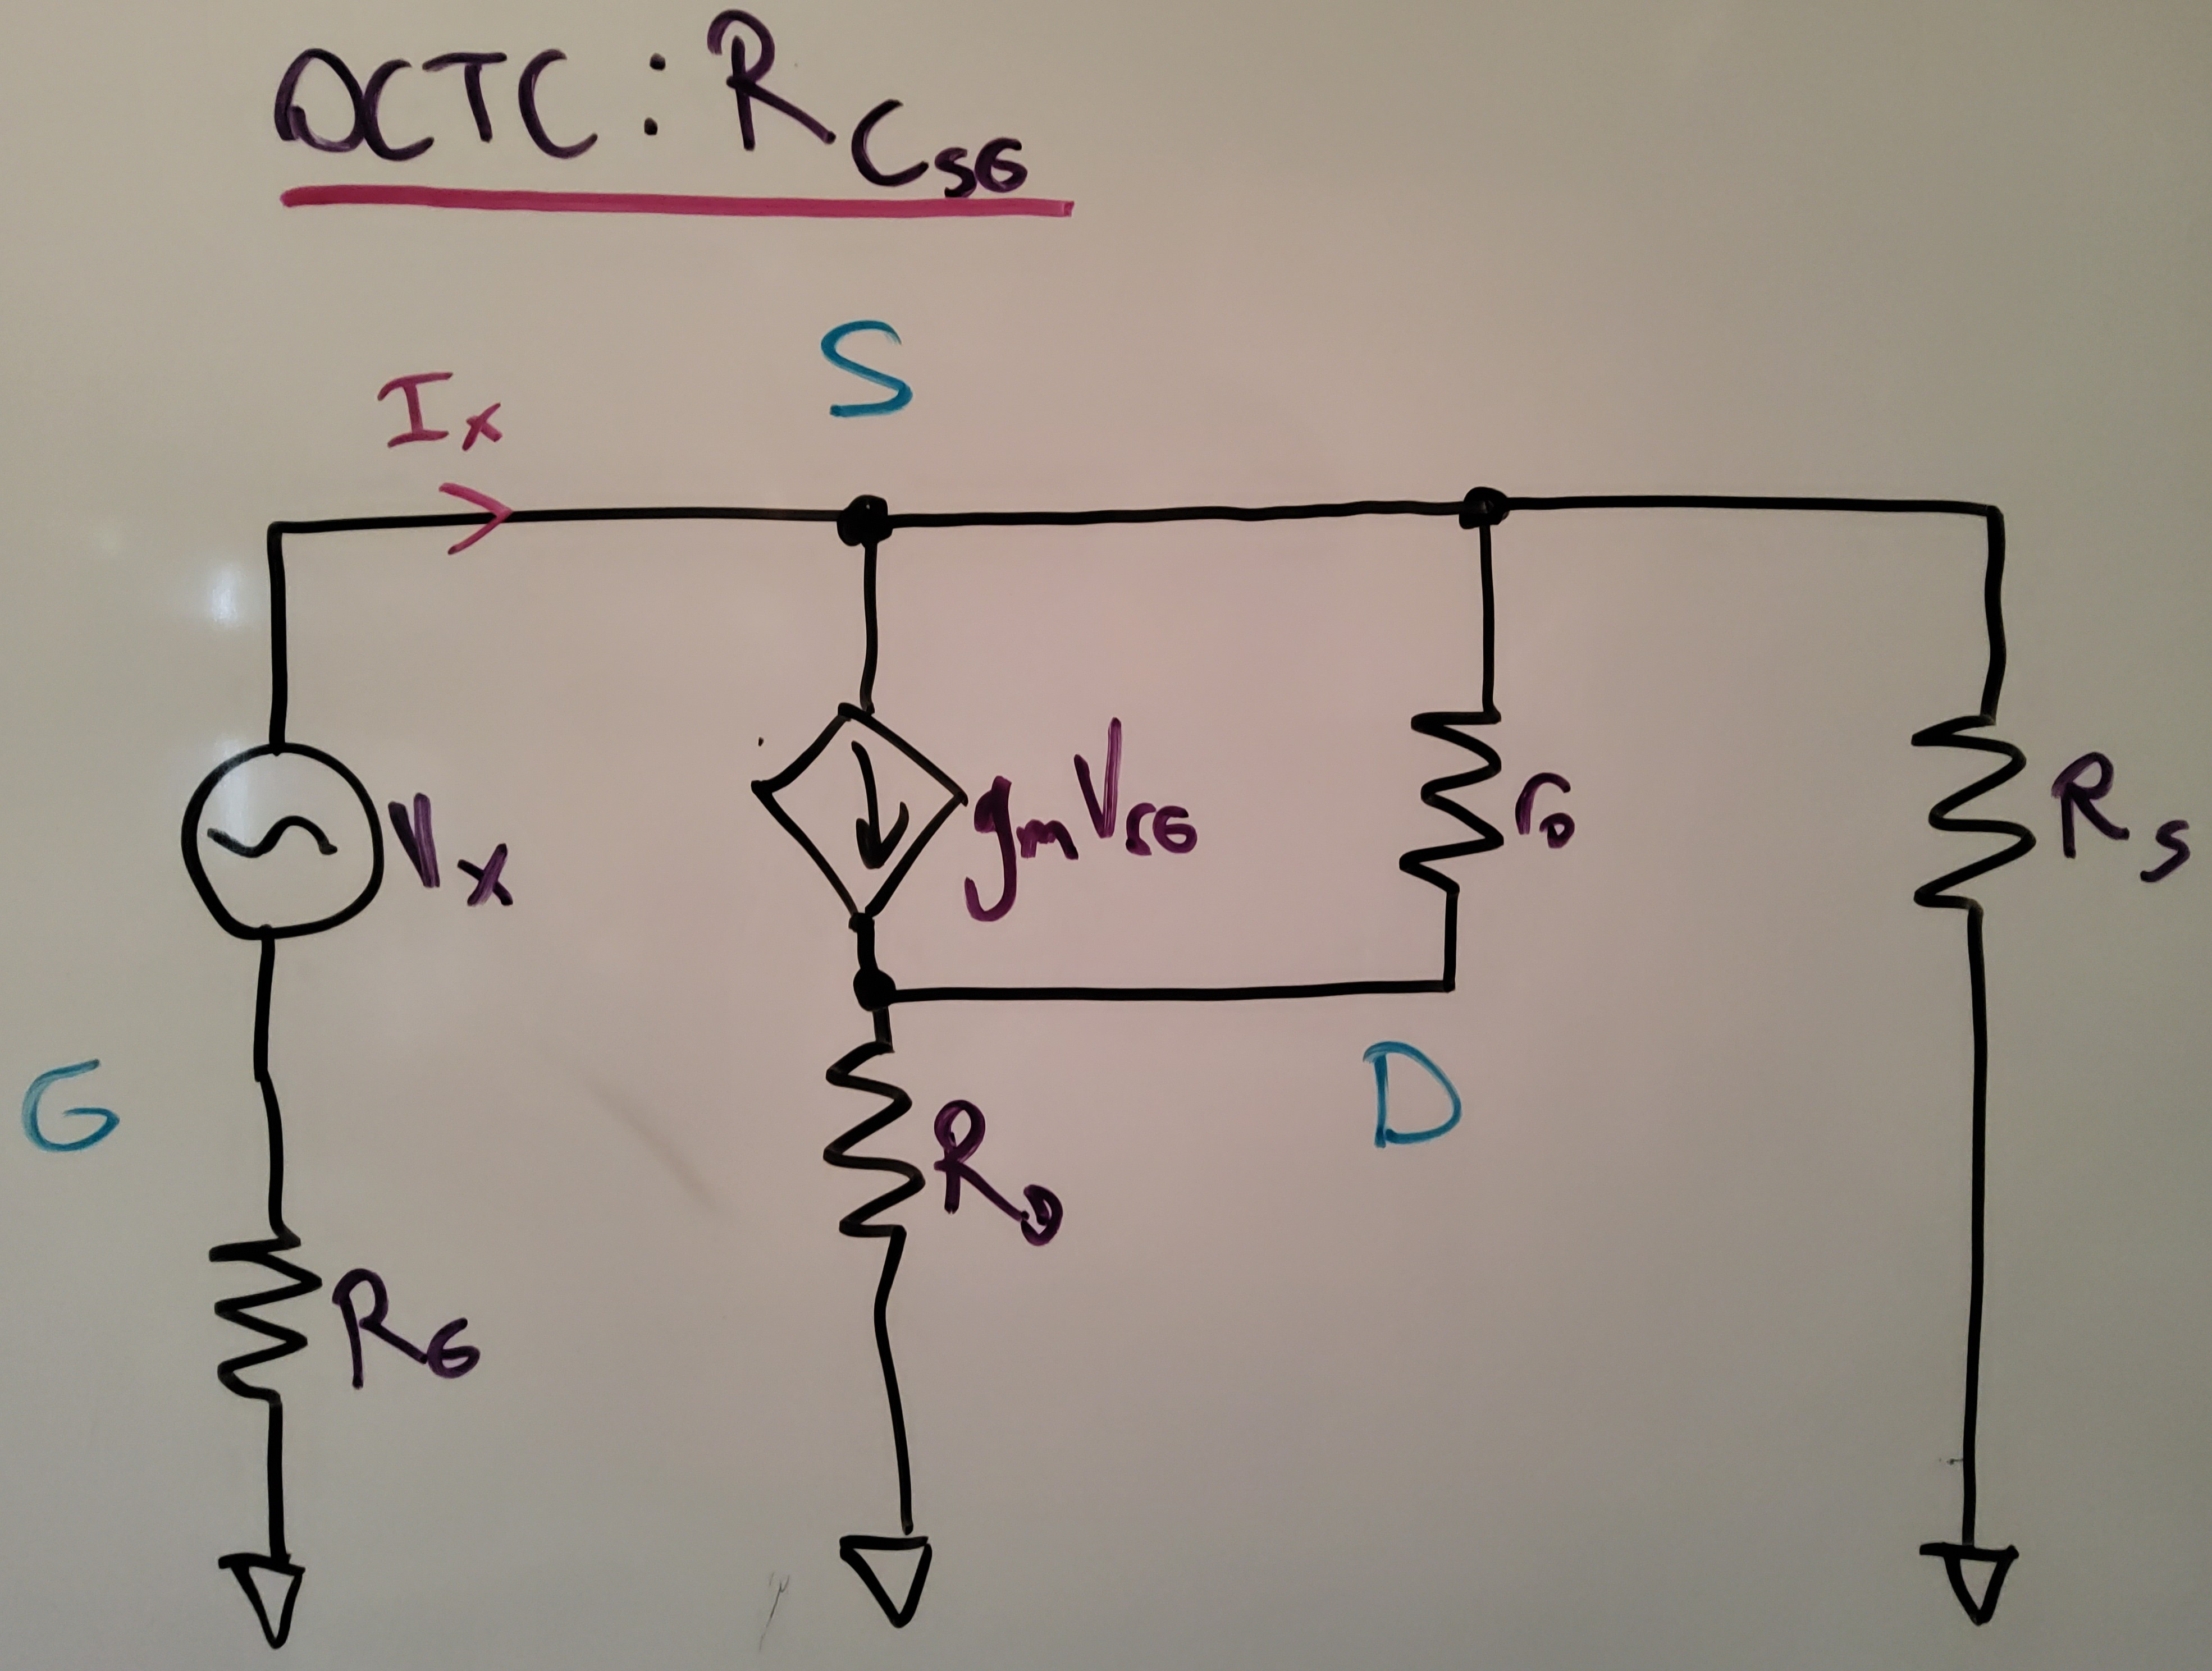
\includegraphics[scale=0.09, center]{p3c_sg.jpg}\\
    }

    We can see that $V_S$ = $V_X$, but with two unknown voltages, we will need three equations.  Analysis of the model yields:
    \begin{align}
        I_X &= -\frac{V_G}{R_G}\\[0.25cm]
        \implies V_G  &= -(I_X \cdot R_G)
        \label{eq:csg1}\\[0.25cm]
        I_X &= g_m V_{XG} + \frac{V_{XD}}{r_o} + \frac{V_X}{R_S}
        \label{eq:csg2}\\[0.25cm]
        0 &= \frac{V_D}{R_D} + \frac{V_{DX}}{r_o} - g_m V_{XG}
        \label{eq:csg3}
    \end{align}

    First let's rearrange \textit{Eq.~\ref{eq:csg3}}, and substitute in \textit{Eq.~\ref{eq:csg1}}
    \begin{align}
        \frac{V_D}{R_D} + \frac{V_{DX}}{r_o} - g_m V_{XG}
        &= V_D\left(\frac{1}{R_D} + \frac{1}{r_o}\right) - \frac{V_X}{r_o} - g_m V_X + g_m V_G\\[0.25cm]
        \implies V_D &= r_o \parallel R_D \left[V_X\left(\frac{1}{r_o} + g_m\right) - g_m V_G\right]\\[0.25cm]
        &= r_o \parallel R_D \left[V_X\left(\frac{1}{r_o} + g_m\right) - g_m (-I_X \cdot R_G)\right]
        \label{eq:csg4}
    \end{align}

\newpage

    Now let's work with \textit{Eq.~\ref{eq:csg2}}, substituting in both \textit{Eq.~\ref{eq:csg1}} and \textit{Eq.~\ref{eq:csg4}} when necessary:
    \begin{align*}
        I_X &= g_m V_X - g_m V_G + \frac{V_X}{r_o} - \frac{V_D}{r_o} + \frac{V_X}{R_S}\\[0.25cm]
        &= V_X \left(g_m + \frac{1}{r_o} + \frac{1}{R_S}\right) - g_m (-I_X \cdot R_G) - \frac{V_D}{r_o}\\[0.25cm]
        &= V_X \left(\frac{r_o + R_S + g_m r_o R_S}{r_o R_S}\right)\\[0.25cm]
            &\qquad - \frac{1}{r_o}\left(r_o \parallel R_D \left[V_X\left(\frac{1}{r_o} + g_m\right) + I_X g_m R_G\right]\right)
            + I_X g_m R_G\\[0.25cm]
        &= V_X \left(\frac{r_o + R_S + g_m r_o R_S}{r_o R_S}\right)\\[0.25cm]
            &\qquad - V_X \left[\frac{R_D}{r_o + R_D}\left(\frac{1 + g_m r_o}{r_o}\right)\right]
            - I_X g_m R_G\left(\frac{R_D}{r_o + R_D}\right)
            + I_X g_m R_G\\[0.25cm]
        &= V_X \left[\left(\frac{r_o + R_S + g_m r_o R_S}{r_o R_S}\right)
            - \frac{R_D}{r_o + R_D}\left(\frac{1 + g_m r_o}{r_o}\right)\right]\\[0.25cm]
            &\qquad - I_X \left[ g_m R_G\left(\frac{R_D}{r_o + R_D}\right) - g_m R_G \right]\\[0.25cm]
        \implies &\; I_X\left[1 + g_m R_G \left(\frac{R_D}{r_o + R_D} -  1\right)\right]\\[0.25cm]
        &\qquad = V_X \left[\frac{(r_o + R_D)(r_o + R_S + g_m r_o R_S) - R_S R_D(1 + g_m r_o)}{r_o R_S(r_o + R_D)}\right]\\[0.35cm]
        \implies \frac{V_X}{I_X} &= \mathlarger{\mathlarger{\frac{\frac{r_o + R_D + g_m R_G R_D - g_m R_G(r_o + R_D)}{\cancel{r_o + R_D}}}{\frac{(r_o + R_D)(r_o + R_S + g_m r_o R_S) - R_S R_D(1 + g_m r_o)}{r_o R_S\cancel{(r_o + R_D)}}}}}\\[0.25cm]
        \implies R_{C_{SG}} &= \frac{r_o R_S\left[r_o + R_D + g_m R_G R_D - g_m R_G(r_o + R_D)\right]}{(r_o + R_D)(r_o + R_S + g_m r_o R_S) - R_S R_D(1 + g_m r_o)}
    \end{align*}

    Since we assume that $R_G = 0$, the equation simplifies to:
    \begin{equation}
        \boxed{R_{C_{SG}} = \frac{r_o R_S}{(r_o + R_S + g_m r_o R_S) - \mathlarger{\frac{R_S R_D(1 + g_m r_o)}{r_o + R_D}}}}
    \end{equation}
\newpage

    \newpage
    \underline{\textbf{OCTC: $C_{DG}$}}\\[0.1cm]
    Below is a schematic of the small-signal model, with all caps opened, and a test source applied in place of $C_{DG}$.  As noted previously, we assume that $R_G = 0$, so we will treat it as a wire to simplify the calculations:

    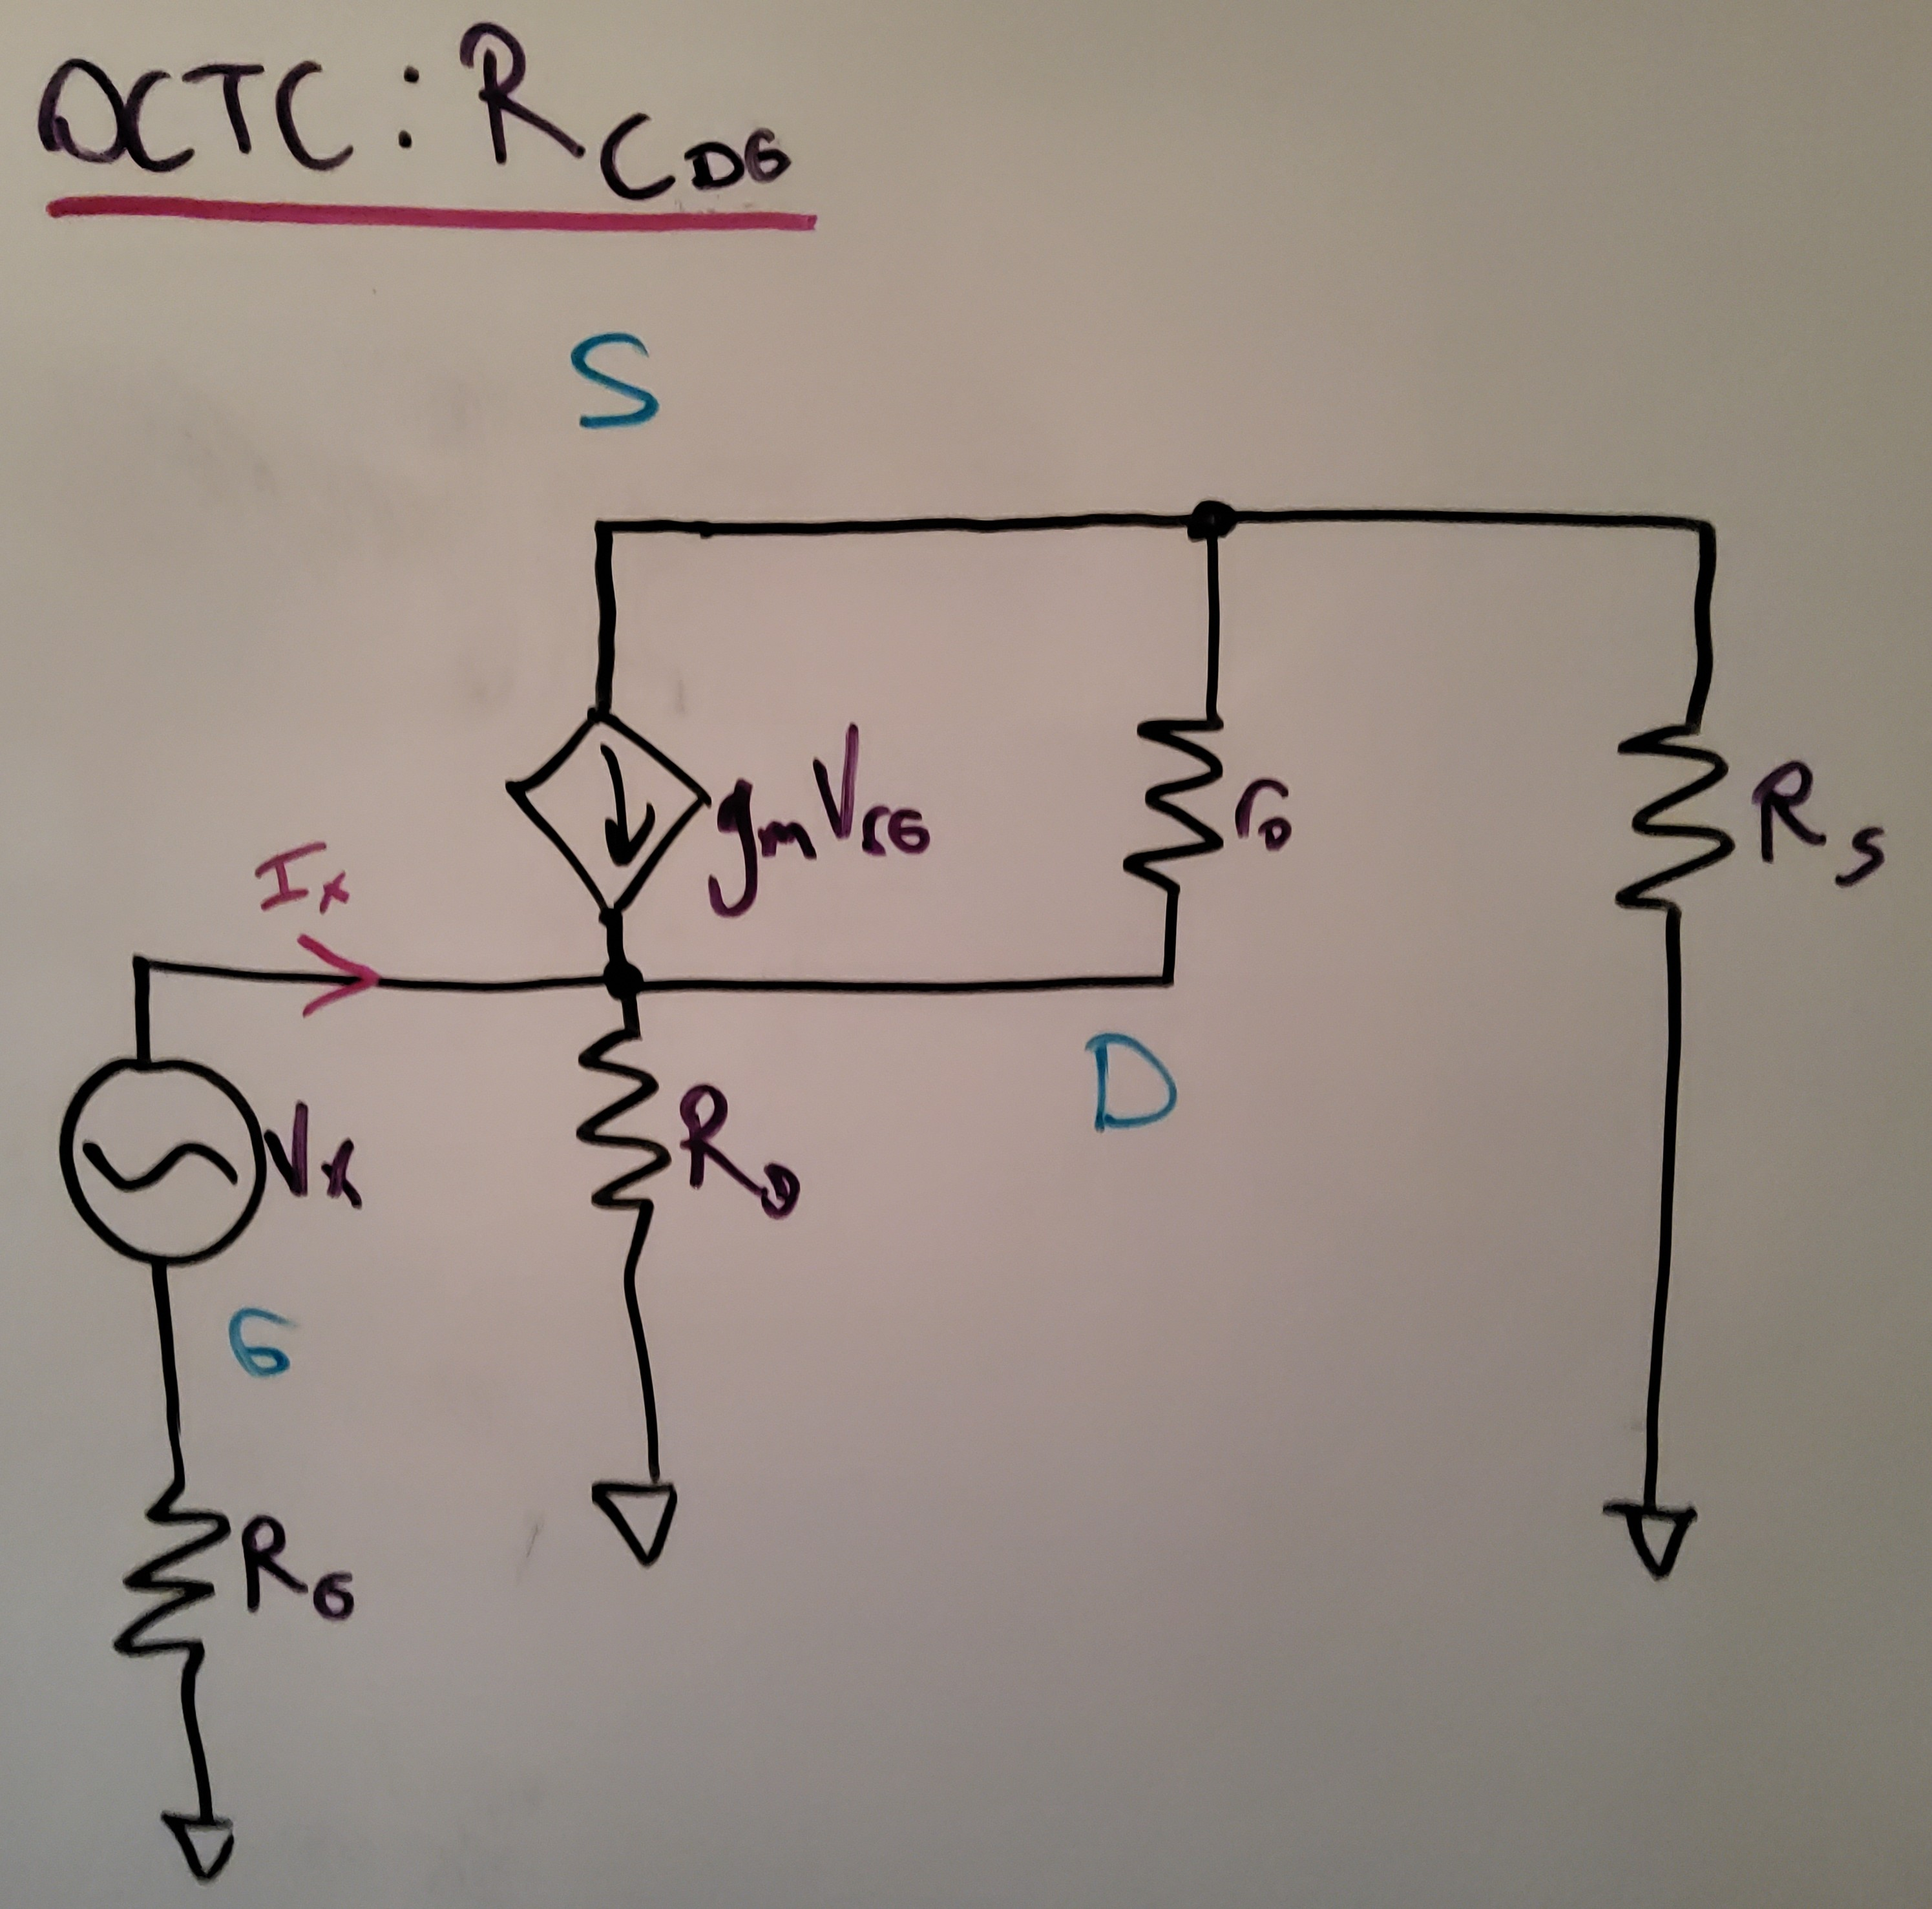
\includegraphics[scale=0.12, center]{p3c_dg.jpg}\\
    
    We note that $V_D = V_X$ and $V_G = 0$.  Then we have two equations:
    \begin{align}
        I_X &= \frac{V_S}{R_S}\\[0.25cm]
        \implies V_S  &= I_X \cdot R_S
        \label{eq:cdg1}\\[0.25cm]
        I_X &= \frac{V_X}{R_D} + g_m V_S + \frac{V_{XS}}{r_o}
        \label{eq:cdg2}
    \end{align}
\newpage
    Rearranging \textit{Eq.~\ref{eq:cdg2}}, and substituting in \textit{Eq.~\ref{eq:cdg1}}
    \begin{align*}
        I_X &= V_X \left(\frac{1}{R_D} + \frac{1}{r_o}\right) - V_S \left(g_m + \frac{1}{r_o}\right)\\[0.25cm]
        &= V_X \left(\frac{1}{R_D} + \frac{1}{r_o}\right) - (I_X \cdot R_S) \left(g_m + \frac{1}{r_o}\right)\\[0.25cm]
        \implies &\; I_X \left[1 +  R_S\left(g_m + \frac{1}{r_o}\right)\right]= V_X \left(\frac{1}{R_D} + \frac{1}{r_o}\right)\\[0.25cm]
        \implies \; \Aboxed{R_{C_{DG}} &= r_o \parallel R_D \left[1 +  R_S\left(g_m + \frac{1}{r_o}\right)\right]}
    \end{align*}

    Now we can find the $-3\,dB$ bandwidth by summing up the circuit time constants and taking its inverse:
    \begin{align*}
        \sum_{i=i}^{n - 1} \tau_i &= (R_{C_{SG}} C_{SG}) + (R_{C_{DG}} C_{DG})\\[0.25cm]
        &= \left(C_{SG} \cdot \frac{r_o R_S}{(r_o + R_S + g_m r_o R_S) - \mathlarger{\frac{R_S R_D(1 + g_m r_o)}{r_o + R_D}}}\right)\\[0.25cm]
        &\qquad + \left(C_{DG}\cdot r_o \parallel R_D \left[1 +  R_S\left(g_m + \frac{1}{r_o}\right)\right]\right)\\[0.25cm]
    \end{align*}
    
    Then our final expression for the $-3\,dB$ bandwidth using OCTC is:
    \begin{equation*}
        \boxed{\mathlarger{\mathlarger{\omega_0 = \frac{1}{\left(\frac{C_{SG}(r_o R_S)}{(r_o + R_S + g_m r_o R_S) - \frac{R_S R_D(1 + g_m r_o)}{r_o + R_D}}\right) + \Bigg(C_{DG} \left(r_o \parallel R_D\right) \Big[1 +  R_S\left(g_m + \frac{1}{r_o}\right)\Big]\Bigg)}}}}
    \end{equation*}
\newpage

    %%%%%%%%%%%%%%%%%%
    %%% SOLUTION C %%%
    %%%%%%%%%%%%%%%%%%
    \item
    {
    First let's derive the mid-band gain of the circuit.  Below is the schematic we will analyze:
    
    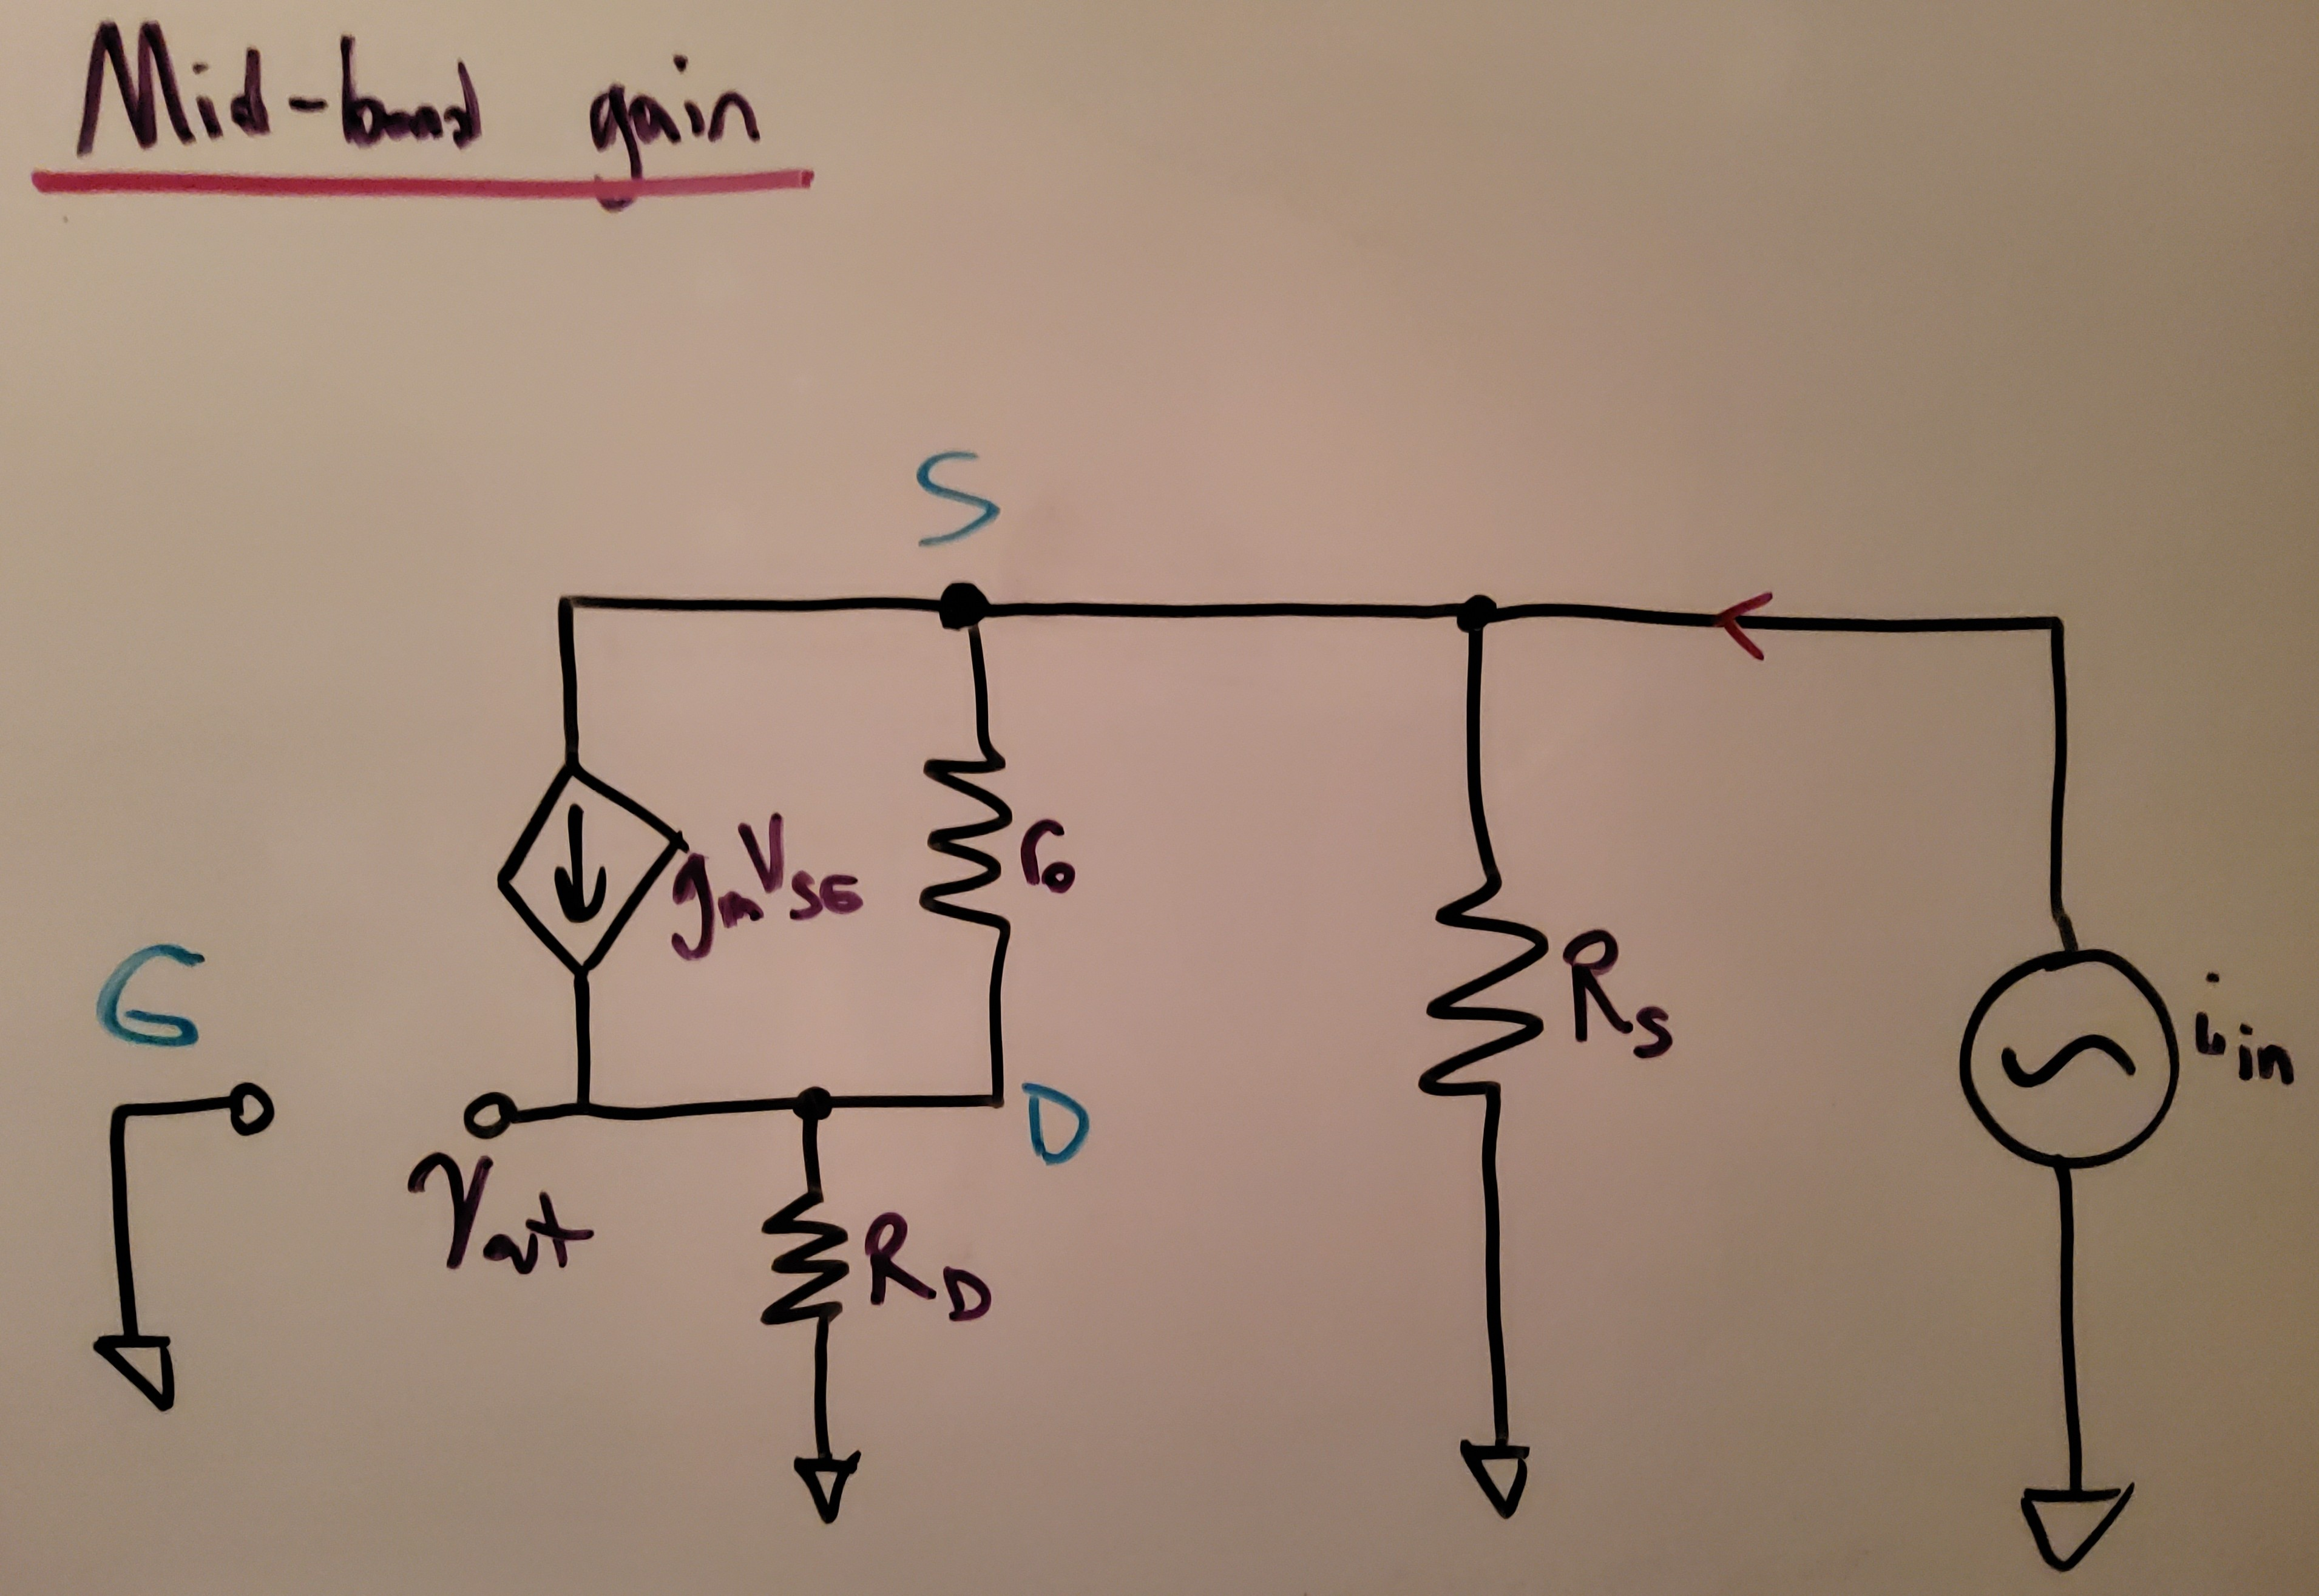
\includegraphics[scale=0.12, center]{p3mbg.jpg}\\
    
    The input current entering the source node is: 
    \begin{align}
        i_{in} &= \frac{V_S}{R_S} + \frac{V_{SD}}{r_o} + g_m V_{SG}\\[0.25cm]
        &= V_S\left(\frac{1}{R_S} + \frac{1}{r_o} + g_m\right) - \frac{V_D}{r_o}
        \label{eq:mbg1}
    \end{align}

    Nodal analysis at the drain node yields: 
    \begin{align}
        0 &= \frac{V_D}{R_D} + \frac{V_{DS}}{r_o} - g_m V_{SG}\\[0.25cm]
        \implies &\; V_S\left(\frac{1}{r_o} + g_m\right) = V_D\left(\frac{1}{r_o} + \frac{1}{R_D}\right)\\[0.25cm]
        \implies &\; V_S = V_D \left(\frac{r_o + R_D}{\cancel{r_o} R_D}\right)\left(\frac{\cancel{r_o}}{1 + g_m r_o}\right)\\[0.25cm]
        \implies &\; V_S = V_D \left(\frac{r_o + R_D}{R_D(1 + g_m r_o)}\right)
        \label{eq:mbg2}
    \end{align}
    }
    
\newpage
    We note that $V_G = 0\,V$, and $V_D = v_{out}$, and substitute \textit{Eq.~\ref{eq:mbg2}} into \textit{Eq.~\ref{eq:mbg1}}:
    Nodal analysis at the drain node yields:
    
    \begin{align*}
        i_{in} &= \left[v_{out} \left(\frac{r_o + R_D}{R_D(1 + g_m r_o)}\right)\right]\left(\frac{1}{R_S} + \frac{1}{r_o} + g_m\right) - \frac{v_{out}}{r_o}\\[0.25cm]
        &= v_{out} \left[\left(\frac{r_o + R_D}{R_D(1 + g_m r_o)}\right)\left(\frac{r_o + R_S + g_m r_o R_S}{r_o R_S}\right) - \frac{1}{r_o}\right]\\[0.25cm]
        &= v_{out} \left[\left(\frac{r_o + R_D(r_o + R_S + g_m r_o R_S)}{r_o R_S R_D(1 + g_m r_o)}\right) - \frac{R_S R_D(1 + g_m r_o)}{r_o R_S R_D (1 + g_m r_o)}\right]\\[0.25cm]
    \end{align*}

    Then we have an expression for the gain of this transimpedance amplifier:
    \begin{equation}
        \boxed{A_i = \frac{v_{out}}{i_{in}} = \frac{r_o R_S R_D (1 + g_m r_o)}{r_o + R_D(r_o + R_S + g_m r_o R_S) - R_S R_D(1 + g_m r_o)}}
    \end{equation}
    
    Since we want to see how the gain responds to different values of $R_S$, let's factor it out of the equation to get a better idea:
    \begin{equation}
        A_i = \frac{R_S}{R_S}\left[\frac{r_o R_D (1 + g_m r_o)}{\frac{r_o}{R_S} + R_D(\frac{r_o}{R_S} + 1 + g_m r_o) - R_D(1 + g_m r_o)}\right]
    \end{equation}
    
    There are two terms with $R_S$ in the denominator that decrease as $R_S$ increases.  Since these are individual sum terms in the denominator, the overall gain will increase with everything else held constant.  Thus, we want to maximize the value of $R_S$ while keeping the amplifier in saturation.\\[0.5cm]
    This can be seen intuitively by looking at the schematic.  If $R_S = 0$, then the input current is shorted to ground in AC, and there would be no signal at the output.  With $R_S = \infty$, all of $i_{in}$ reaches $v_{out}$, and we would have maximum gain.  Then we must consider the maximum value of $R_S$ that would not take the transistor out of saturation.

    %%%%%%%%%%%%%%%%%%
    %%% SOLUTION D %%%
    %%%%%%%%%%%%%%%%%%
    \item
    {
    Any positive value of $R_G$ will decrease the bandwidth, due to the gate being tied to $C_{DG}$ and $C_{SG}$.  Thus, to maximize the bandwidth of the amplifier we want $\boxed{R_G = 0}$
    }
\end{enumerate}
\newpage
%%%%%%%%%%%%%%%%%%%%%%%%%%%%%%%%%%%%%%%%%%%%%%%%%%%%%%%%%%%%%%%%%%%%%%%%%%%%%%%%%%%%%%%%%%%%%%%%%%%%%%%%%%%
%                                             APPENDIX                                                    %
%%%%%%%%%%%%%%%%%%%%%%%%%%%%%%%%%%%%%%%%%%%%%%%%%%%%%%%%%%%%%%%%%%%%%%%%%%%%%%%%%%%%%%%%%%%%%%%%%%%%%%%%%%%
\appendix
%%%%%%%%%%%%%%%%%%%%%%%%%%%%%%%%%%%%%%%%%%%%%%%%%%%%%%%%%%%%%%%%%%%%%%%%%%%%%%%%%%%%%%%%%%%%%%%%%%%%%%%%%%%
%                                APPENDIX A: GLOSSARY OF EQUATIONS                                        %
%%%%%%%%%%%%%%%%%%%%%%%%%%%%%%%%%%%%%%%%%%%%%%%%%%%%%%%%%%%%%%%%%%%%%%%%%%%%%%%%%%%%%%%%%%%%%%%%%%%%%%%%%%%
\newpage
\section{Appendix: Glossary of Equations}
    \begin{flalign}
        &&\Aboxed{\phi_{bi} &= \frac{kT}{q} \cdot ln\;\bigg( \frac{N_D \cdot N_A}{{n_i}^2} \bigg)}
        &&\textit{Built-in potential, $PN$-junction}
        \label{eq:phi_bi}
    \end{flalign}

    \begin{flalign}
        &&\Aboxed{W_{dep} &= \sqrt{\frac{2\epsilon_s \left(\phi_{bi} - V_{applied}\right)}{q}
                        \cdot \Bigg( \frac{1}{N_A} + \frac{1}{N_D} \Bigg)}}
        &&\textit{Depletion region width, total}
        \label{eq:total_dep}
    \end{flalign}        

    \begin{flalign}
        &&\Aboxed{C_{dep} &= A \left(\frac{\epsilon_s}{W_{dep}}\right)}
        &&\textit{Junction capacitance}
        \label{eq:junc_cap}
    \end{flalign}

    \begin{flalign}
        &&\Aboxed{I_{DS,sat} &= \left(\frac{W}{2L}\right) \mu_n\,C_{ox}
                         {\big(V_{GS} - V_{T_n}\big)}^2 (1 + \lambda V_{DS})}
        &&\textit{$NMOS$ saturation current}
        \label{eq:mosfet_ids_nmos_sat}\\[0.25cm]
        &&\Aboxed{I_{DS,tri} &= \left(\frac{W}{L}\right) \mu_n\,C_{ox}
                            \left(V_{GS} - V_{T_n} - \frac{V_{DS}}{2}\right) V_{DS}}
        &&\textit{$NMOS$ triode current}
        \label{eq:mosfet_ids_nmos_tri}\\[0.25cm]
        &&\Aboxed{I_{SD,sat} &= \left(\frac{W}{2L}\right) \mu_p\,C_{ox}
                         {\big(V_{SG} - \left|V_{T_p}\right|\big)}^2 (1 + \lambda V_{SD})}
        &&\textit{$PMOS$ saturation current}
        \label{eq:mosfet_ids_pmos_sat}\\[0.25cm]
        &&\Aboxed{I_{SD,tri} &= \left(\frac{W}{L}\right) \mu_p\,C_{ox}
                            \left(V_{SG} - \left|V_{T_p}\right| - \frac{V_{SD}}{2}\right) V_{SD}}
        &&\textit{$PMOS$ triode current}
        \label{eq:mosfet_ids_pmos_tri}
    \end{flalign}

    \begin{flalign}
        &&\Aboxed{r_o &= \frac{1}{\frac{W\,\mu\,C_{ox}}{2L}{(V_{GS} - V_T)}^2\,\lambda}
        \approx \frac{1}{\lambda\,I_{DS}}}
        &&\textit{Output resistance for MOSFET}
        \label{eq:mos_outresistance}
    \end{flalign}

    \begin{flalign}
        &&\Aboxed{g_m &= \left(\frac{W}{L}\right)\mu\,C_{ox}(V_{{DS}_{sat}})
        = \sqrt{\left(\frac{2W}{L}\right)\mu\,C_{ox} I_{DS}}
        = \frac{2 \cdot I_{DS}}{V_{GS} - V_T}}
        &&\textit{Transconductance for MOSFET}
        \label{eq:mos_transconductance}
    \end{flalign}

    \begin{flalign}
        &&\Aboxed{V_{GS} = V_T + \sqrt{\frac{2\,I_{DS}}{\frac{W}{L} \mu C_{ox}}} = V_T + V_{OD}}
        &&\textit{Gate-source condition, diode-connected MOSFET}
        \label{eq:mos_gate_cond}
    \end{flalign}
%%%%%%%%%%%%%%%%%%%%%%%%%%%%%%%%%%%%%%%%%%%%%%%%%%%%%%%%%%%%%%%%%%%%%%%%%%%%%%%%%%%%%%%%%%%%%%%%%%%%%%%%%%%
%                                APPENDIX B: GLOSSARY OF TABLES                                           %
%%%%%%%%%%%%%%%%%%%%%%%%%%%%%%%%%%%%%%%%%%%%%%%%%%%%%%%%%%%%%%%%%%%%%%%%%%%%%%%%%%%%%%%%%%%%%%%%%%%%%%%%%%%
\newpage
\section{Appendix: Glossary of Tables}
    \begin{table}[H]
    \centering
    \setlength{\tabcolsep}{20pt}
    \renewcommand{\arraystretch}{1.5}
    \begin{tabular}{|l|c|c|c|}
        \hline
        \textbf{Transistor Type}  &  \textbf{Cut-off} & \textbf{Triode} & \textbf{Saturation}\\
        \hline
        \textit{NMOS} & $V_{GS} \leq V_{T_n}$
                        & $V_{DS} \leq V_{GS} - V_{T_n}$
                        & $V_{DS} > V_{GS} - V_{T_n}$\\
        \hline
        \textit{PMOS} & $V_{SG} \leq \left|V_{T_p}\right|$
                        & $V_{SD} \leq V_{SG} - \left|V_{T_p}\right|$
                        & $V_{SD} > V_{SG} - \left|V_{T_p}\right|$\\
        \hline
    \end{tabular}
    \caption{Conditions for MOSFET regions of operation.
    \label{tab:mosfet_op}} 
    \end{table}

    \begin{table}[H]
    \centering
    \setlength{\tabcolsep}{20pt}
    \renewcommand{\arraystretch}{1.5}
    \begin{tabular}{|l|c|c|}
        \hline
        \textbf{Description}  &  \textbf{Symbol} & \textbf{Value}\\
        \hline
        Elementary charge & $q$ & $\num{1.60218e-19}\,C$\\
        \hline
        Electron volt & $eV$ & $\num{1.60218e-19}\,J$\\
        \hline
        Boltzmann's constant & $k$ & $\num{1.38066e-23}\,J/K$\\
        \hline
        Free electron mass & $m_0$ & $\num{9.1095e-31}\,kg$\\
        \hline
        Permittivity in vacuum & $\epsilon_0$ & $\num{8.85418e-12}\,F/m$\\
        \hline
        Planck's constant & $h$ & $\num{6.62617e-34}\,J \cdot s$\\
        \hline
        Reduced Planck's constant ($h/2\pi$) & $\hbar$ & $\num{1.05458e-34}\,J \cdot s$\\
        \hline
        Speed of light in vacuum & $c$ & $\num{2.99792e8}\,m/s$\\
        \hline
        Thermal voltage at $T=300^{\circ}K$ & $kT/q$ & $0.0259\,V$\\
        \hline
        Wavelength of 1-$eV$ photon & $\lambda$ & $1.23977\,\mu m$\\
        \hline
    \end{tabular}
    \caption{Physical constants.
    \label{tab:phys_const}} 
    \end{table}
\newpage
    \begin{table}[H]
    \centering
    \setlength{\tabcolsep}{20pt}
    \renewcommand{\arraystretch}{1.5}
    \begin{tabular}{|l|c|c|}
        \hline
        \textbf{Quantity}  &  \textbf{Symbol} & \textbf{Value/Dimension}\\
        \hline
        Meter & $m$ & $1\,m = 10^2\,cm$\\
        \hline
        Millimeter & $mm$ & $1\,mm = 10^{-1}\,cm = 10^{-3}\,m$\\
        \hline
        Micrometer, micron & $\mu m$ & $1\,\mu m = 10^4\,\text{\AA} = 10^3\,mm = 10^{-4}\,cm$\\
        \hline
        Nanometer & $nm$ & $1\,nm = 10\,\text{\AA} = 10^{-3}\,\mu m = 10^{-7}\,cm$\\
        \hline
        Angstrom & $\text{\AA}$ & $1\,\text{\AA} = 10^{-4}\,\mu m = 10^{-8}\,cm = 10^{-10}\,m$\\
        \hline
        Electron volt & $eV$ & $1\,eV = \num{1.60218e-19}\,J$\\
        \hline
        Electric charge (Coulomb) & $C$ & $A \cdot s$\\
        \hline
        Current (Ampere) & $A$ & $C/s$\\
        \hline
        Frequency (Hertz) & $Hz$ & $1/s$\\
        \hline
        Energy (Joule) & $J$ & $N \cdot m$\\
        \hline
        Power (Watt) & $W$ & $J/s$\\
        \hline
        Potential (Volt) & $V$ & $J/C$\\
        \hline
        Conductance (Siemens) & $S$ & $A/V$\\
        \hline
        Resistance (Ohm) & $\Omega$ & $V/A$\\
        \hline
        Capacitance (Farad) & $F$ & $C/V$\\
        \hline
    \end{tabular}
    \caption{Unit conversions.
    \label{tab:unit_conv}} 
    \end{table}
\newpage
%%%%%%%%%%%%%%%%%%%%%%%%%%%%%%%%%%%%%%%%%%%%%%%%%%%%%%%%%%%%%%%%%%%%%%%%%%%%%%%%%%%%%%%%%%%%%%%%%%%%%%%%%%%
%                                           BIBLIOGRAPHY                                                  %
%%%%%%%%%%%%%%%%%%%%%%%%%%%%%%%%%%%%%%%%%%%%%%%%%%%%%%%%%%%%%%%%%%%%%%%%%%%%%%%%%%%%%%%%%%%%%%%%%%%%%%%%%%%
\newpage
\addcontentsline{toc}{section}{References}
\emergencystretch=2em
\nocite{*}
\printbibliography
%%%%%%%%%%%%%%%%%%%%%%%%%%%%%%%%%%%%%%%%%%%%%%%%%%%%%%%%%%%%%%%%%%%%%%%%%%%%%%%%%%%%%%%%%%%%%%%%%%%%%%%%%%%
%                                           END OF DOCUMENT                                               %
%%%%%%%%%%%%%%%%%%%%%%%%%%%%%%%%%%%%%%%%%%%%%%%%%%%%%%%%%%%%%%%%%%%%%%%%%%%%%%%%%%%%%%%%%%%%%%%%%%%%%%%%%%%
\end{document}
